%% Follow comments to support use.

%%%%%%%%%%%%%%%%%%%%%%%%%%%%%%%%%%%%%%%%%%%%%%%%%%%%%%%%%
%% STEP 1: Choose options for MSc / BSc / seminar layout and your bibliographic style
%%%%%%%%%%%%%%%%%%%%%%%%%%%%%%%%%%%%%%%%%%%%%%%%%%%%%%%%%

%%  Language: 
%%      finnish, swedish, or english
%%  Pagination (use twoside by default)  
%%      oneside or twoside,
%%  Study programme / kind of report
%%      csm  = Master's thesis in Computer Science Master's Programme;
%%      tkt = Bachelor's thesis in Computer Science Bachelor's Programme;
%%      seminar = seminar report
%%  For Master's thesis choose your line or track:
%%      (30 cr thesis, 2020 onwards, Master's Programme in Computer Science = csm)
%%      software-track-2020 = Software study track
%%      algorithms-track-2020 = Algorithms study track
%%      networking-track-2020 = Networking study track

\documentclass[english,twoside,censored,tkt]{HYthesisML} 


% If wanted, open new chapters only at right page.
% By default, "openany".
%\PassOptionsToClass{openright,twoside,a4paper}{report}
\PassOptionsToClass{openany,twoside,a4paper}{report}

\usepackage{csquotes}
%%%%%%%%%%%%%%%%%%%%%%%%%%%%%%%%%%%%%%%%%%%%%%%%%%%%%%%%%
%% REFERENCES
%% Some notes on bibliography usage and options:
%% natbib -> you can use, e.g., \citep{} or \parencite{} for (Einstein, 1905); with APA \cite -> Einstein, 1905 without ()
%% maxcitenames=2 -> only 2 author names in text citations, if more -> et al. is used
%% maxbibnames=99 as no great need to suppress the biliography list in a thesis
%% for more information see biblatex package documentation, e.g., from https://ctan.org/pkg/biblatex 

%% Reference style: select one 
%% for APA = Harvard style = authoryear -> (Einstein, 1905) use:
\usepackage[style=authoryear,bibstyle=authoryear,backend=biber,natbib=true,maxnames=99,maxcitenames=2,uniquelist=minyear,giveninits=true,uniquename=mininit]{biblatex}
%% for numeric = Vancouver style -> [1] use:
%\usepackage[style=numeric,bibstyle=numeric,backend=biber,natbib=true,maxbibnames=99,giveninits=true,uniquename=init]{biblatex}
%% for alpahbetic -> [Ein05] use:
%\usepackage[style=alphabetic,bibstyle=alphabetic,backend=biber,natbib=true,maxbibnames=99,giveninits=true,uniquename=init]{biblatex}
%

\addbibresource{bibliography.bib}
% in case you want the final delimiter between authors & -> (Einstein & Zweistein, 1905) 
% \renewcommand{\finalnamedelim}{ \& }
% List the authors in the Bibilipgraphy as Lastname F, Familyname G,
\DeclareNameAlias{sortname}{family-given}
% remove the punctuation between author names in Bibliography 
%\renewcommand{\revsdnamepunct}{ }


%% Block of definitions for fonts and packages for picture management.
%% In some systems, the figure packages may not be happy together.
%% Choose the ones you need.

%\usepackage[utf8]{inputenc} % For UTF8 support, in some systems. Use UTF8 when saving your file.
\usepackage{multirow}
\usepackage{lmodern}         % Font package, again in some systems.
\usepackage{textcomp}        % Package for special symbols
\usepackage[pdftex]{color, graphicx} % For pdf output and jpg/png graphics
\usepackage{epsfig}
\usepackage{subfigure}
\usepackage[pdftex, plainpages=false]{hyperref} % For hyperlinks and pdf metadata
\usepackage{fancyhdr}        % For nicer page headers
\usepackage{tikz}            % For making vector graphics (hard to learn but powerful)
%\usepackage{wrapfig}        % For nice text-wrapping figures (use at own discretion)
\usepackage{amsmath, amssymb} % For better math


\singlespacing               %line spacing options; normally use single

\fussy
%\sloppy                      % sloppy and fussy commands can be used to avoid overlong text lines
% if you want to see which lines are too long or have too little stuff, comment out the following lines
% \overfullrule=1mm
% to see more info in the detailed log about under/overfull boxes...
% \showboxbreadth=50 
% \showboxdepth=50



%%%%%%%%%%%%%%%%%%%%%%%%%%%%%%%%%%%%%%%%%%%%%%%%%%%%%%%%%
%% STEP 2:
%%%%%%%%%%%%%%%%%%%%%%%%%%%%%%%%%%%%%%%%%%%%%%%%%%%%%%%%%
%% Set up personal information for the title page and the abstract form.
%% Replace parameters with your information.
\title{Multimodal Machine Learning and Data Fusion in Medical Diagnosis}

\author{Juuso Saavalainen}
\date{\today}

% Set supervisors, use the titles according to the thesis language
% in English Prof. or Dr., or in Finnish toht. or tri or FT, TkT, Ph.D. or in Swedish... 
\supervisors{Prof.~Ville~Mustonen, Ph.D. student~Teemu~Kuosmanen}

\keywords{Deep learning, Multimodal learning, Data fusion}
\additionalinformation{\translate{\track}}

%% For seminar reports:
%%\additionalinformation{Name of the seminar}

%% Provide classification terms, to appear on the abstract page.
%% Replace the classification terms below with the ones that match your work.
%% ACM Digital library provides a taxonomy and a tool for classification
%% in computer science. Use 1-3 paths, and use right arrows between the
%% about three levels in the path; each path requires a new line.

\classification{\protect{\ \\
\  Applied computing $\rightarrow$ Life and medical sciences  $\rightarrow$ Health informatics\  \\
\  Computing methodologies  $\rightarrow$ Machine learning  $\rightarrow$ Machine learning approaches $\rightarrow$ Neural networks
}}

%% If you want to quote someone special. You can comment this line out and there will be nothing on the document.
%\quoting{Bachelor's degrees make pretty good placemats if you get them laminated.}{Jeph Jacques}


%% OPTIONAL STEP: Set up properties and metadata for the pdf file that pdfLaTeX makes.
%% Your name, work title, and keywords are recommended.
\hypersetup{
    unicode=true,           % to show non-Latin characters in Acrobat’s bookmarks
    pdftoolbar=true,        % show Acrobat’s toolbar?
    pdfmenubar=true,        % show Acrobat’s menu?
    pdffitwindow=false,     % window fit to page when opened
    pdfstartview={FitH},    % fits the width of the page to the window
    pdftitle={},            % title
    pdfauthor={},           % author
    pdfsubject={},          % subject of the document
    pdfcreator={},          % creator of the document
    pdfproducer={pdfLaTeX}, % producer of the document
    pdfkeywords={something} {something else}, % list of keywords for
    pdfnewwindow=true,      % links in new window
    colorlinks=true,        % false: boxed links; true: colored links
    linkcolor=black,        % color of internal links
    citecolor=black,        % color of links to bibliography
    filecolor=magenta,      % color of file links
    urlcolor=cyan           % color of external links
}

%%-----------------------------------------------------------------------------------

\begin{document}

% Generate title page.
\maketitle

%%%%%%%%%%%%%%%%%%%%%%%%%%%%%%%%%%%%%%%%%%%%%%%%%%%%%%%%%
%% STEP 3:
%%%%%%%%%%%%%%%%%%%%%%%%%%%%%%%%%%%%%%%%%%%%%%%%%%%%%%%%%
%% Write your abstract in the separate file, to be positioned here.
%% You can make several abstract pages (if you want it in different languages),
%% in which case you should also define the language of the abstract,
%% as below.

% \begin{abstract}{finnish}

% Tämä dokumentti on tarkoitettu Helsingin yliopiston tietojenkäsittelytieteen osaston opin\-näyt\-teiden ja harjoitustöiden ulkoasun ohjeeksi ja mallipohjaksi. Ohje soveltuu kanditutkielmiin, ohjelmistotuotantoprojekteihin, seminaareihin ja maisterintutkielmiin. Tämän ohjeen lisäksi on seurattava niitä ohjeita, jotka opastavat valitsemaan kuhunkin osioon tieteellisesti kiinnostavaa, syvällisesti pohdittua sisältöä.


% Työn aihe luokitellaan  
% ACM Computing Classification System (CCS) mukaisesti, 
% ks.\ \url{https://dl.acm.org/ccs}. 
% Käytä muutamaa termipolkua (1--3), jotka alkavat juuritermistä ja joissa polun tarkentuvat luokat erotetaan toisistaan oikealle osoittavalla nuolella.

% \end{abstract}

\begin{otherlanguage}{english}
\begin{abstract}

Traditionally machine learning models are build to take use of single modality. Medical diagnosis is rarely based on single source of information. Multimodal machine learning  introduces techniques like data fusion that allow models to process and use multiple modalities. This thesis examines these models in a context of medical diagnosing. 

Multiple recent literature reviews suggest potential improvements in accuracy with multimodal machine learning compared to the models utilizing single modality in the same task. However, most of the research in this area is found employing retrospective data and lack prospective validation. 

The thesis follows a structure that aims to first provide overview of the basics in machine and deep learning. Then it moves to examine data fusion and medical studies employing multimodal machine learning.  

\end{abstract}
\end{otherlanguage}

\chapter*{Tiivistelmä}
Nyky-yhteiskunnassa kerätään ja tallennetaan tietoa ennennäkemättömin määrin. Tämä tarjoaa merkittäviä mahdollisuuksia koneoppimiselle (Machine Learning) ja tekoälylle (Artificial Intelligence). Koneoppimisen sovellukset ulottuvat lähes kaikialle, terveydenhuolto ja lääketiede mukaan lukien. Neuroverkkojen ja syväoppimismallien kehittyminen on mahdollistanut monimutkaisten ja laajojen tietomassojen analysoinnin. Lääkärit hyödyntävät usein diagnosoinnin tukena useita tietolähteitä kuten kuvia, mittaustuloksia, ja oireita. Diagnoisointiin tai taudin luokan tunnistamiseen kuuluu siten usein monien eri lähteiden datan arvioimista yhtenäisenä kokonaisuutena. Radiologiassa syväoppimista on käytetty esimerkiksi kuvien segmentointiin ja poikkeavuuksien tunnistamiseen (\cite{lee2017deep}). Lupaavista tuloksista huolimatta tekoälyyn pohjautuvien järjestelmien käyttö terveydenhuollossa on vielä olematonta.

Tämän tutkielman tarkoituksena on selvittää ja tutkia miten useita modaliteettäjä hyödynnytään diagnosinnin tukena, mihin ne pohjautuvat sekä mitä ongelmia niiden käyttöön liittyy. Erityisesti tutkielma keskittyy useiden modaliteettien käyttöön liittyvään datafuusioon, eli useiden modaliteettien yhteen sovittamiseen koneoppimis arkkitehtuureissa. Modaliteetillä tarkoitetaan tietotyyppiä kuten kuvaa tai ääntä. Tämän lisäksi tutkielma käsittelee neuroverkkoja ja syväoppimista perusteiden kautta rakentaen pohjan kompleksisempien kokonaisuuksien ja datafuusion käsittelyyn.

Ohjattu oppiminen (Supervised learning) on yksi koneoppimisen osa-alue, jossa olemassa olevan datan avulla pyritään muodostamaan malli, joka pystyy esimerkiksi luokittelemaan sille syötettävää dataa. Ohjattuun oppimiseen tarvitaan siis dataa joka on jo luokiteltua, tätä kutsutaan koulutus dataksi. Lineaarinen regressio on hyvä selkeä esimerkki joka soveltuu yksinkertaisten ongelmien ratkaisemiseen. Datan ulottuvuuksien ja kompleksisuuden lisääntyessä edistyneemmät algoritmit, kuten neuroverkot, toimivat paremmin. 

Neuroverkon rakenne koostuu yksinkertaisimmillaan solmuista, jotka sijaitsevat verkon eri kerroksissa. Kokonaan yhdistetyssä neuroverkossa jokainen solmu yhdistyy jokaiseen seuraavan kerroksen solmuun. Solmujen väliselle yhteydelle sijoittuu paino sekä jokaiseen solmuun harha. Neuroverkon kouluttamisella tarkoitetaankin näiden painojen ja harhojen säätelyä niin, että verkko tuottaa halutun tuloksen. Neuroverkon ensimmäinen kerros jota usein kutsutaan syötekerrokseksi (Input layer) ottaa esimerkiksi kuvan pikselien arvoja solmujen arvoiksi. Kuva, joka koostuu 20x20 pikselistä, tuottaa täten 400 solmun kokoisen syötekerroksen josta jokainen solmu yhdistyy jokaiseen seuraavan kerroksen solmuun. Neuroverkon viimeistä kerrosta kutsutaan tulostekerrokseksi (Output layer) ja sen solmujen määrä määräytyy esimerkiksi luokittelutehtävissä luokiteltavien kohteiden mukaan. Ensimmäisen ja viimeisen kerroksen koko on siis valmiiksi määritelty. Kerroksia jotka sijaitsevat syöte ja tuloste kerroksen välissä kutsutaan piilokerroksiksi (Hidden layer). Piilokerrosten määrää ja kokoa ei ole valmiiksi määritelty, syväoppimisesta puhuttaessa viitataan verkkoihin joissa piilokerroksia on useita. 

Neuroverkkon kouluttamisella tarkoitetaan prosessia jossa verkon harhat ja painot optimoidaan. Koulutukseen käytettävä data voidaan jakaa testi- ja koulutusdataan jolloin verkon suoriutumista voidaan arvioida datalla, jota ei ole käytetty sen kouluttamiseen. Eteenpäinsyöttö algoritmin avulla verkon syöte viedään kerroksien läpi aina tuloste kerrokselle asti. Yksittäisen solmun aktivaatio voidaan laskea siihen kytkettyjen solmujen painolla skaalattujen arvojen summana, johon lisätään solmun harha. Tätä summaa voidaan kutsua solmun lineaariseksi muunnokseksi, jotta aktivaatio saadaan laskettua tähän sovitetaan aktivaatiofunktio. Aktivaatiofunktion avulla lineaarisuus saadaan rikottua. Tämä mahdollistaa epälineaaristen suhteiden mallintamisen. Samalla kaavalla voidaan edetä tuloskerrokselle asti. Tulostekerroksen aktivaatiofunktio poikkeaa usein muiden kerroksien aktivaatiofunktiosta, koska tämän kerroksen arvot halutaan kuvata todennäköisyyksinä ja täten niiden summan on oltava 1. Viimeisen kerroksen solmujen ja syötteen tunnisteen (label) erotusta kutsutaan kustannusfunktioksi. Takaisinvirtausalgortimi hyödyntää tätä ja sen tehtävä on laskea jokaisen painon ja harhan osittaisderivaatta suhteessa kustannusfunktioon. Näitä arvoja voidaan kutsua myös gradienteiksi. Gradientti suhteessa kustannusfunktioon kertoo suunnan, joka kasvattaa sen arvoa nopeimmin. Siirtämällä painoja ja harhoja kohti negatiivistä gradienttiä voidaan kustannusfunktion arvo minimoida. Neuroverkkoja on kehitetty moneen tarkoitukseen. Useat näistä kuten konvoluutio ja takisinkytkentäneuroverkot perustuvat samojen algoritmien ja koulutustekniikoiden käyttöön kuin kokonaan kytketyssä eteenpäinsyöttö neuroverkossa. 

Multimodaalinen koneoppiminen (Multimodal machine learning) pyrkii hyödyntämään useita modaliteettejä saman aikaisesti. Multimodaalista koneoppimista voidaan hyödyntää monissa eri käyttötarkoituksissa kuten generatiivisessä tekoälyssä. Lääketieteellisessä diagnosoinnissa multimodaalisia koneoppimista voidaan hyödyntää esimerkiksi tunnistamaan tauti. Esimerkiksi röntgenkuvien avulla voidaan kouluttaa malli tunnistamaan nivelrikko (\cite{tiulpin2018automatic}). Malleja, jotka pohjautuvat vain yhden modaliteetin kuten kuvan käyttöön, kutsutaan unimodaalisiksi (Unimodal) malleiksi. Röntgenkuvien lisäksi mallille voidaan syöttää myös muita modaliteettejä, jotka ovat relevantteja ongelman kannalta. Esimerkiksi lääketieteellisten kuvien lisäksi voidaan käyttää potilaskertomuksia, mittaus- tai testi tuloksia, tai geneettisiä tietoja. Datafuusio käsittelee useiden modaliteettien yhdistelemistä (\cite{8269806}). Datafuusiomenetelmät voidaan karkeasti jakaa kolmeen luokkaan: aikaiseen , myöhäiseen ja keskivaiheen fuusioon. Mallille syötettävät modaliteetit ovat lähtökohtaisesti erillisiä ja rakenteellisesti toisistaan poikkeavia. Fuusiomenetelmien etuliite kuvaa arkkitehtuurissa fuusion vaiheen ajankohtaa suhteessa koneoppimisalgoritmiin tai -malliin. Aikaisella fuusiolla tarkoitetaan täten siis menetelmää, jossa modaliteetit yhdistetään yhtenäiseksi ennen mallille syöttämistä. Myöhäinen fuusio taas on menetelmä, jossa jokainen modaliteetti käsitellään erillisenä ja jokainen syötetään omaan malliin. Näiden tuloksia yhdistetään ennen lopullista päätöksentekoa. Keskivaiheen fuusiolla tarkoitetaan yhdistämistä, joka tapahtuu mallin sisällä. Kaikista näistä myös löytyy variaatioita, joissa esimerkiksi jokin modaliteetti käsitellään eri tavalla.

Fuusiomenetelmän toimivuuteen vaikuttaa vahvasti ongelma, jota pyritään ratkaisemaan. Lisäksi siihen vaikuttaa datan määrä ja laatu. Aikaisen fuusion menetelmässä voidaan esimerkiksi hyödyntää valmiiksi koulutettuja malleja tai autoenkoodereita (Auto encoder) modaliteettien kuvaamiseksi yhtenäiseksi vektoriksi. Myöhäisen fuusion kohdalla taas voidaan hyödyntää unimodaaleja malleja, joiden koulutus ja käyttö eivät ole sidoksissa muihin modaliteetteihin. Myöhäisen fuusiota hyödyntävissä kokonaisuuksissa voidaan myös puuttuviin modaliteetteihin reagoida, koska yksikään osa ei ole suoraan riippuvainen muista modaliteeteistä. Keskivaiheen fuusio hyödyntää neuroverkkoja ja poiketen muista menetelmistä, se voidaan kouluttaa yhtenäisenä mallina ja takaisinvirtausalgoritmiä hyödyntäen aina tuloksesta alkuperäisiin syötteisiin asti. Neuroverkkojen hyödyntäminen vaatii enemmän dataa kuin muut menetelmät ja tekee siten mallin kouluttamisesta vaikempaa. Tieteellisessä yhteisössä ei ole konsensusta siitä, mikä menetelmistä on tehokkain. Multimodaaliseen koneoppimiseen liittyvät keskeiset haasteet voidaan jakaa viiteen luokkaan (\cite{8269806}):

\textbf{1.} \textit{Esittäminen (Representation)} miten useat modaliteetit esitetään merkityksellisesti?

\textbf{2.} \textit{Kääntäminen (Translation)} miten data määritetään modaliteetista (A) -> (B)?

\textbf{3.} \textit{Kohdistaminen (Alignment)} mitkä osat yhdestä modaliteetista vastaavat suoraan toista?

\textbf{4.} \textit{Fuusio (Fusion)} miten modaliteetit yhdistetään?

\textbf{5.} \textit{Yhteisoppiminen (Co-learning)} miten tietoa voidaan jakaa eri modaliteettien välillä?

Multimodaaliseen koneoppimiseen pohjautuvien mallien tehokkuuden arviointia vaikeuttaa ratkaisujen vahva riippuvuus käsiteltävästä ongelmasta ja saatavilla olevasta datasta. Monet tutkimukset käyttävät valmiiksi kerättyä dataa, joka ei ole julkisesti saatavilla. Multimodaalista koneoppimista täsmälääketieteessä tarkasteleva kirjallisuuskatsaus (\cite{articlePreciRev}), osoitti usean modaliteetin nostavan mallien tarkkuutta keskimäärin 6.4\% verrattaen yhden modaliteetin malleihin. Katsaukseen päätyneissä artikkeleissä suurimpina ongelmina nousivat pienet otoskoot, luokkien erisuuruus ja retrospektiivinen data. Lisäksi useat tutkimukset käyttivät vain yhden sairaanhoitopiirin dataa. Kliinisen validaation sekä mallien yleistyvyyden arviointiin ei siis tämän katsauksen perusteella pystytä. Huomioitavaa on kuitenkin multimodaalisten mallien tarkkuuden paraneminen verratten vain yhden modaliteetin hyödyntämiseen. Katsaukseen valituista papereissa lääketieteellisistä alueista neurologia ja syöpä olivat eniten edustettuina. Sähköisten terveystiedot ja kuvantamisdata olivat eniten edustettu yhdistelmä modaliteettejä.

Tekoälyn soveltaminen lääketieteellisessä kliinisessä kontekstissa on laaja ongelma. Multimodaalisen datan käyttöön pohjautuvat mallit ovat antaneet lupaavaa näyttöä mahdollisesta tarkkuuden paranemisesta verrattaessa yhden modaliteetin malleihin. Koneoppimiseen pohjautuvien järjestelmien läpinäkyvyydellä ja päätösten selitettävyydellä on merkittävä rooli, kun ajatellaan potentiaalista kliinistä käyttöä.

% Place ToC
%\newpage
\mytableofcontents

\mainmatter

%%%%%%%%%%%%%%%%%%%%%%%%%%%%%%%%%%%%%%%%%%%%%%%%%%%%%%%%%
%% STEP 4: Write the thesis.
%%%%%%%%%%%%%%%%%%%%%%%%%%%%%%%%%%%%%%%%%%%%%%%%%%%%%%%%%
%% Your actual text starts here. You shouldn't mess with the code above the line except
%% to change the parameters. Removing the abstract and ToC commands will mess up stuff.
%%
%% Command \include{file} includes the file of name file.tex.
%% A new page will be created at every \include command, 
%% which makes it appropriate to use it for large entities such as book chapters. Cannot be nested.
%% It is useful for a big project, as changing one of the include targets 
%% won't force the regeneration of the outputs of all the rest.
%% Alternatively, \input is a more lower level macro 
%% which simply inputs the content of the given file like it was copy&pasted there manually.

\chapter{Introduction\label{intro}}

Diagnosing diseases or conditions is a typical task for physicians working in healthcare. Physicians use relevant data that describe the medical condition of the patient. The data needed depends heavily on the context but can be simplified as using the current and historical data available to identify the disease or condition. Additional data can be gathered from medical imaging or lab tests (\cite{NAP21794}). The complexity of the diagnosing process varies case by case but can be seen as a classification problem in the end. 

Machine learning has been used across different industries to solve classification problems, and deep learning has shown potential for complex classification tasks. The capability of the machine learning model is highly dependent on the data that it is trained with. Deep learning has been successfully used for image segmentation and classification in radiology (\cite{lee2017deep}). In medicine, data with multiple modalities namely electronic health records (EHR) and medical images are used together to gain a better understanding of the patient during the diagnostic process. However, machine learning models traditionally expect data from a single modality. Multimodal machine learning (MML) addresses the issue by introducing data fusion for multiple different sources of modalities during the training process (\cite{8269806}).


This thesis provides a basic view of the concepts in multimodal data fusion. This is achieved by introducing basic machine and deep learning concepts and then moving to data fusion. These concepts are then reviewed through recent studies utilizing the multimodal approach in medical contexts. This thesis tries to identify the potential benefits and challenges that can be found from using multiple modalities compared to single-modality approaches. 

\bigskip

\textbf{Research Questions:}

\begin{enumerate}
    \item What are the basic principles of multimodal machine learning and data fusion?
    \item How do recent studies employing multimodal machine learning techniques in medical contexts demonstrate the potential advantages and challenges compared to single-modality approaches?
\end{enumerate}
\chapter{Machine learning methods\label{methods}}

This thesis focuses on supervised machine learning models used in classification problems. Some non-supervised techniques to reduce dimensionality are also introduced. Supervised learning is a type of machine learning in witch the model is trained with labeled data. Formally, a training dataset with $n$ samples can be described as a set of feature vectors $X$ and a corresponding set of labels $Y$: 
\[X = \{ \mathbf{x}_1, \mathbf{x}_2, \ldots, \mathbf{x}_n \} \text{ , } Y = \{ y_1, y_2, \ldots, y_n \}\]
where each feature vector $\mathbf{x}_i$ is a $d$-dimensional vector:
\(\mathbf{x}_i = (x_{i1}, x_{i2}, \ldots, x_{id})\).
The $d$ indicates the number of features per sample. The goal in classification is to create a model that can assign a correct label $y$ to unseen feature vector $\mathbf{x}_i \notin X$.

This chapter follows mainly the ideas presented in a book: \textit{Deep Learning} (\cite{Goodfellow-et-al-2016}). In this chapter, we define some of the fundamental algorithms and methods that are necessary to understand before moving into more complex (MML) models that utilize many data modalities simultaneously. 

\section{Artificial neural networks and deep learning}

Deep learning, or artificial neural networks with multiple layers, has improved performance in multiple machine learning domains like computer vision and natural language processing (\cite{biglecun}). The ability to automatically discover abstract representations from data allows complex functions to be learned (\cite{biglecun}).

The basic structure of the neural network is a set of layers with an input layer, \(n\) hidden layers, and an output layer. Components of these layers are nodes, also referred to as neurons. The idea for the node and the whole fundamental structure of what later evolved to artificial neural networks, is a perceptron that was introduced by \citep{Rosenblatt1958ThePA}. Research for artificial neural networks was already hot in 1980 due to the discovery of key algorithms such as backpropagation (\cite{KARHUNEN2015125}). Interest was declining until deep learning was introduced by \cite{hinton2006fast}, combined with increasing computing power and data amounts (\cite{biglecun}). This can be seen as the starting point for modern deep learning architectures. 

At the input level of a multilayer perceptron (MLP), nodes represent the features that are input to the network. Similarly, the output layer is a set of nodes representing the possible labels in the dataset. For example, identifying a single number when we have 20x20 pixels defining a picture and labels that correspond to that number (1-9), the neural network for this task would have an input layer with 400 nodes and an output layer with 9 nodes. Hidden layers are the layers between the input and output layers. The number of nodes in each hidden layer, and the number of hidden layers are not fixed, like input and output layers. In a fully connected feedforward network (FFNN), all of the nodes per layer are connected with some set of weights and biases to each node in the next layer. In these kinds of networks, the number of weights between layers \({1} \text{ and } {2} \text{ is }  n_{1} \times n_{2}\), where \(n\) represents the number of nodes per layer. Each node, excluding the input layer, also has some bias associated with it. 


\subsection{Forward propagation}

Forward propagation defines the actions that have to be made when feeding data from the input layer through the network. This is done to produce the output layer, which predicts the label corresponding to the input data. The first step in the data flow through the network is to calculate the linear transformation for the nodes in the next layer. With \(n\) input features in FFNN, the linear transformation for a single neuron in the first hidden layer can be defined as
\[z = \sum_{i = 1}^{n} (w_{i} \times x_{i}) + bias\]
where \(w\) represents weight and \(x\) a value associated with a node in the input layer or activation in the previous layer. Activation of a node is then calculated by applying the activation function to the \(z\). Dataflow through a single node is illustrated in Figure {\ref{fig:singlenode}}. The activation function is applied to break the linearity. There are many options when choosing an activation function,  
\[\mathrm{Sigmoid}(z) = {\frac{1}{1+e^{-z}}}
\text{ and }    
\mathrm{RelU}(z) = \begin{cases}
 &x \text{ if } z > 0\\ 
 &0 \text{ otherwise } 
\end{cases}\]
are common, many others are based on these with some modification. For the output layer, a representation that can be viewed as probabilities is wanted. The sum of the activations in the output layer is 1 and each node can get a value in the range [0,1]. This is achieved by applying a softmax activation function to the linear transformation of each node in the output layer. With \(n\) nodes in the output layer softmax of the linear transformations \(z = \{ {z}_1, {z}_2, \ldots,{z}_n \}\) can be calculated as:

\[\mathrm{Softmax}(z_{i}) = \frac{e^{z_{i}}}{\sum_{j=1}^{n}e^{z_{j}}}\]

Forward propagation can be seen as an algorithm that produces the output vector containing the label probabilities with a given input vector X based on the weights and biases of the neural network by feeding the data through the network and calculating the activations for each layer iteratively. The structure of a node or neuron and the idea of activation can be seen influenced by human brains (\cite{Rosenblatt1958ThePA}). Forward propagation is sometimes misunderstood as part of backpropagation, but it is an own separate algorithm.

\begin{figure}
    \centering
    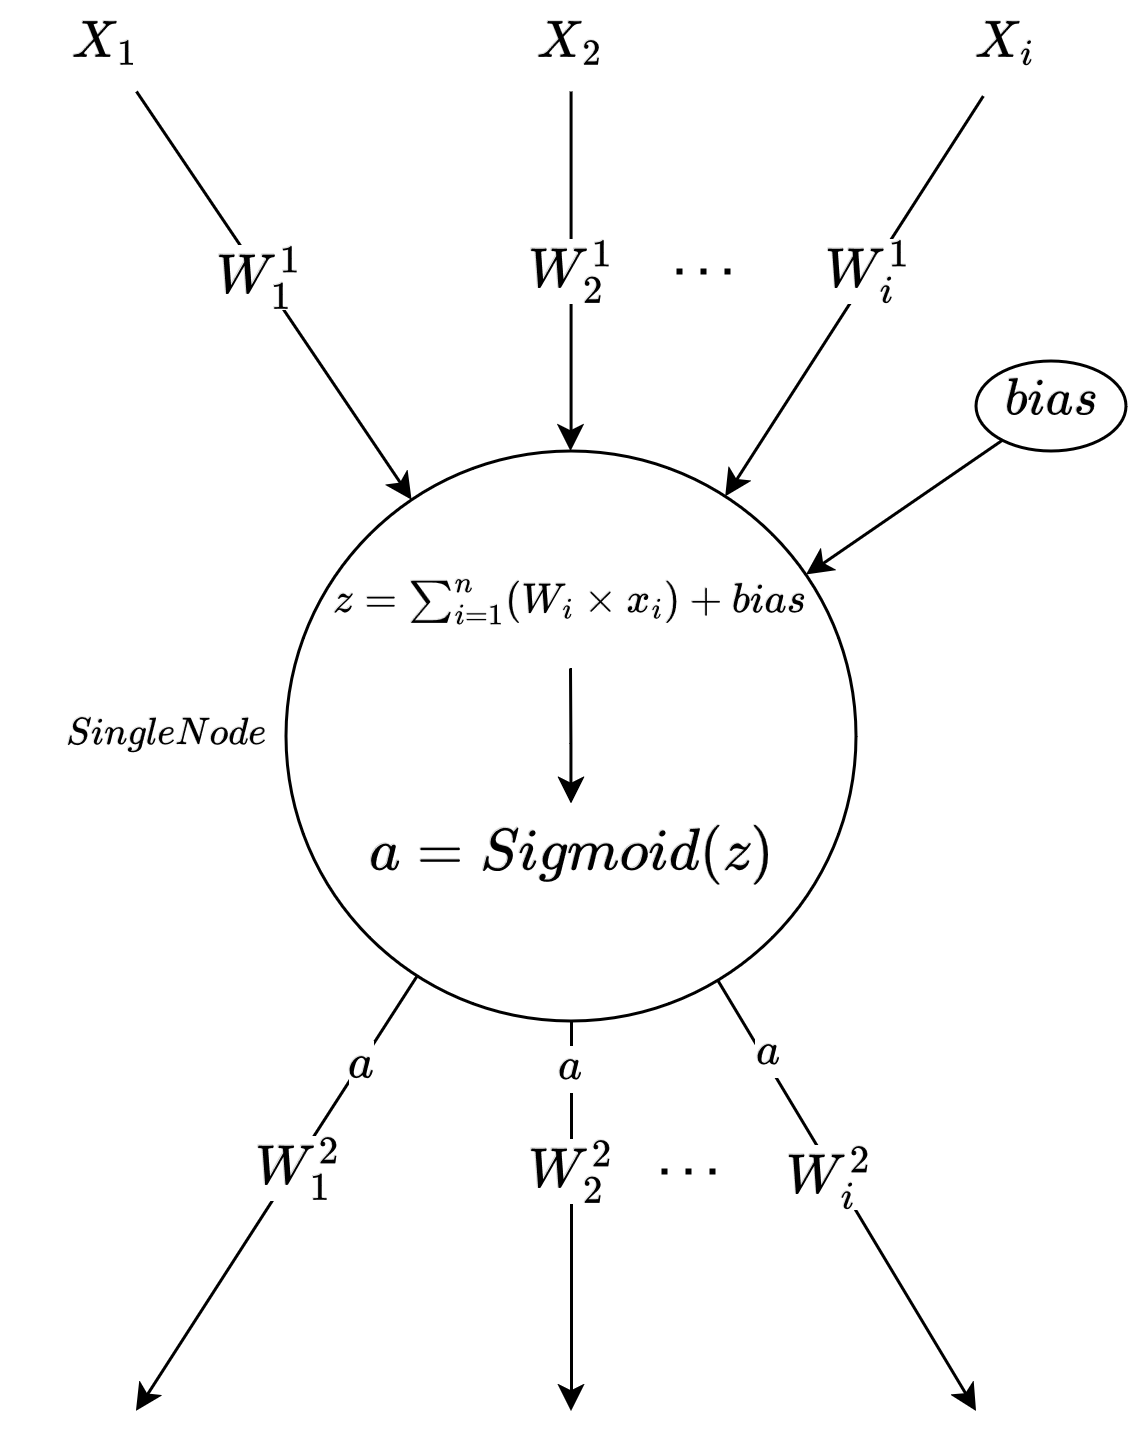
\includegraphics[width=0.5\linewidth]{template//figures/singlenode.png}
    \caption{Forward propagation zoomed in single node}
    \label{fig:singlenode}
\end{figure}


\subsection{Backpropagation}

The mathematical concept of backpropagation was first introduced as a reverse mode of automatic differentiation without direct use of neural networks (\cite{linna}). Later as a part of training the neural networks referred to as backpropagation. With forward propagation, we can produce outputs of the neural network. Backpropagation is an algorithm that is used to find the impact of each weight and bias term on the prediction error. Prediction error, also known as the loss or cost function, defines the disparity between the predicted and desired output. As the correct label is often presented as a single numerical value it needs to be converted into a similar representation as the output of the network. This can be done with one-hot encoding. A single sample from a dataset with 9 possible classes: \(\hat{y} = \{ {0.12}_1, {0.02}_2, \ldots,{0.33}_9 \}\) where the correct label is 2, can be one-hot encoded to \(y = \{ {0}_1, {1}_2, \ldots,{0}_9 \}\). There are multiple ways of calculating the difference or loss between the correct label and the predicted one. One of them is cross-entropy which is suitable for multiclass classification. 
\[\mathrm{CE}(y,\hat{y}) = -\sum_{l}^{L} y_{l} \log(\hat{y}_{l})\]

With backpropagation, we calculate the gradients of the loss function with respect to weights and bias terms. Backpropagation is sometimes misunderstood as the algorithm that optimizes the network (\cite{Goodfellow-et-al-2016}). The gradients can be thought of as a partial derivatives in a vector. We calculate these gradients for each layer moving backward from the output towards the input layer by layer. This is done because, with this approach we can use the chain rule to effectively use the already calculated values from previous layers to reduce the computation time. Backpropagation in FFNN multiclass classification with two input features, two hidden layers, and three output classes is illustrated in \ref{fig:backprop}, where \(L\) is used as the notation for the loss.

\begin{figure}
    \centering
    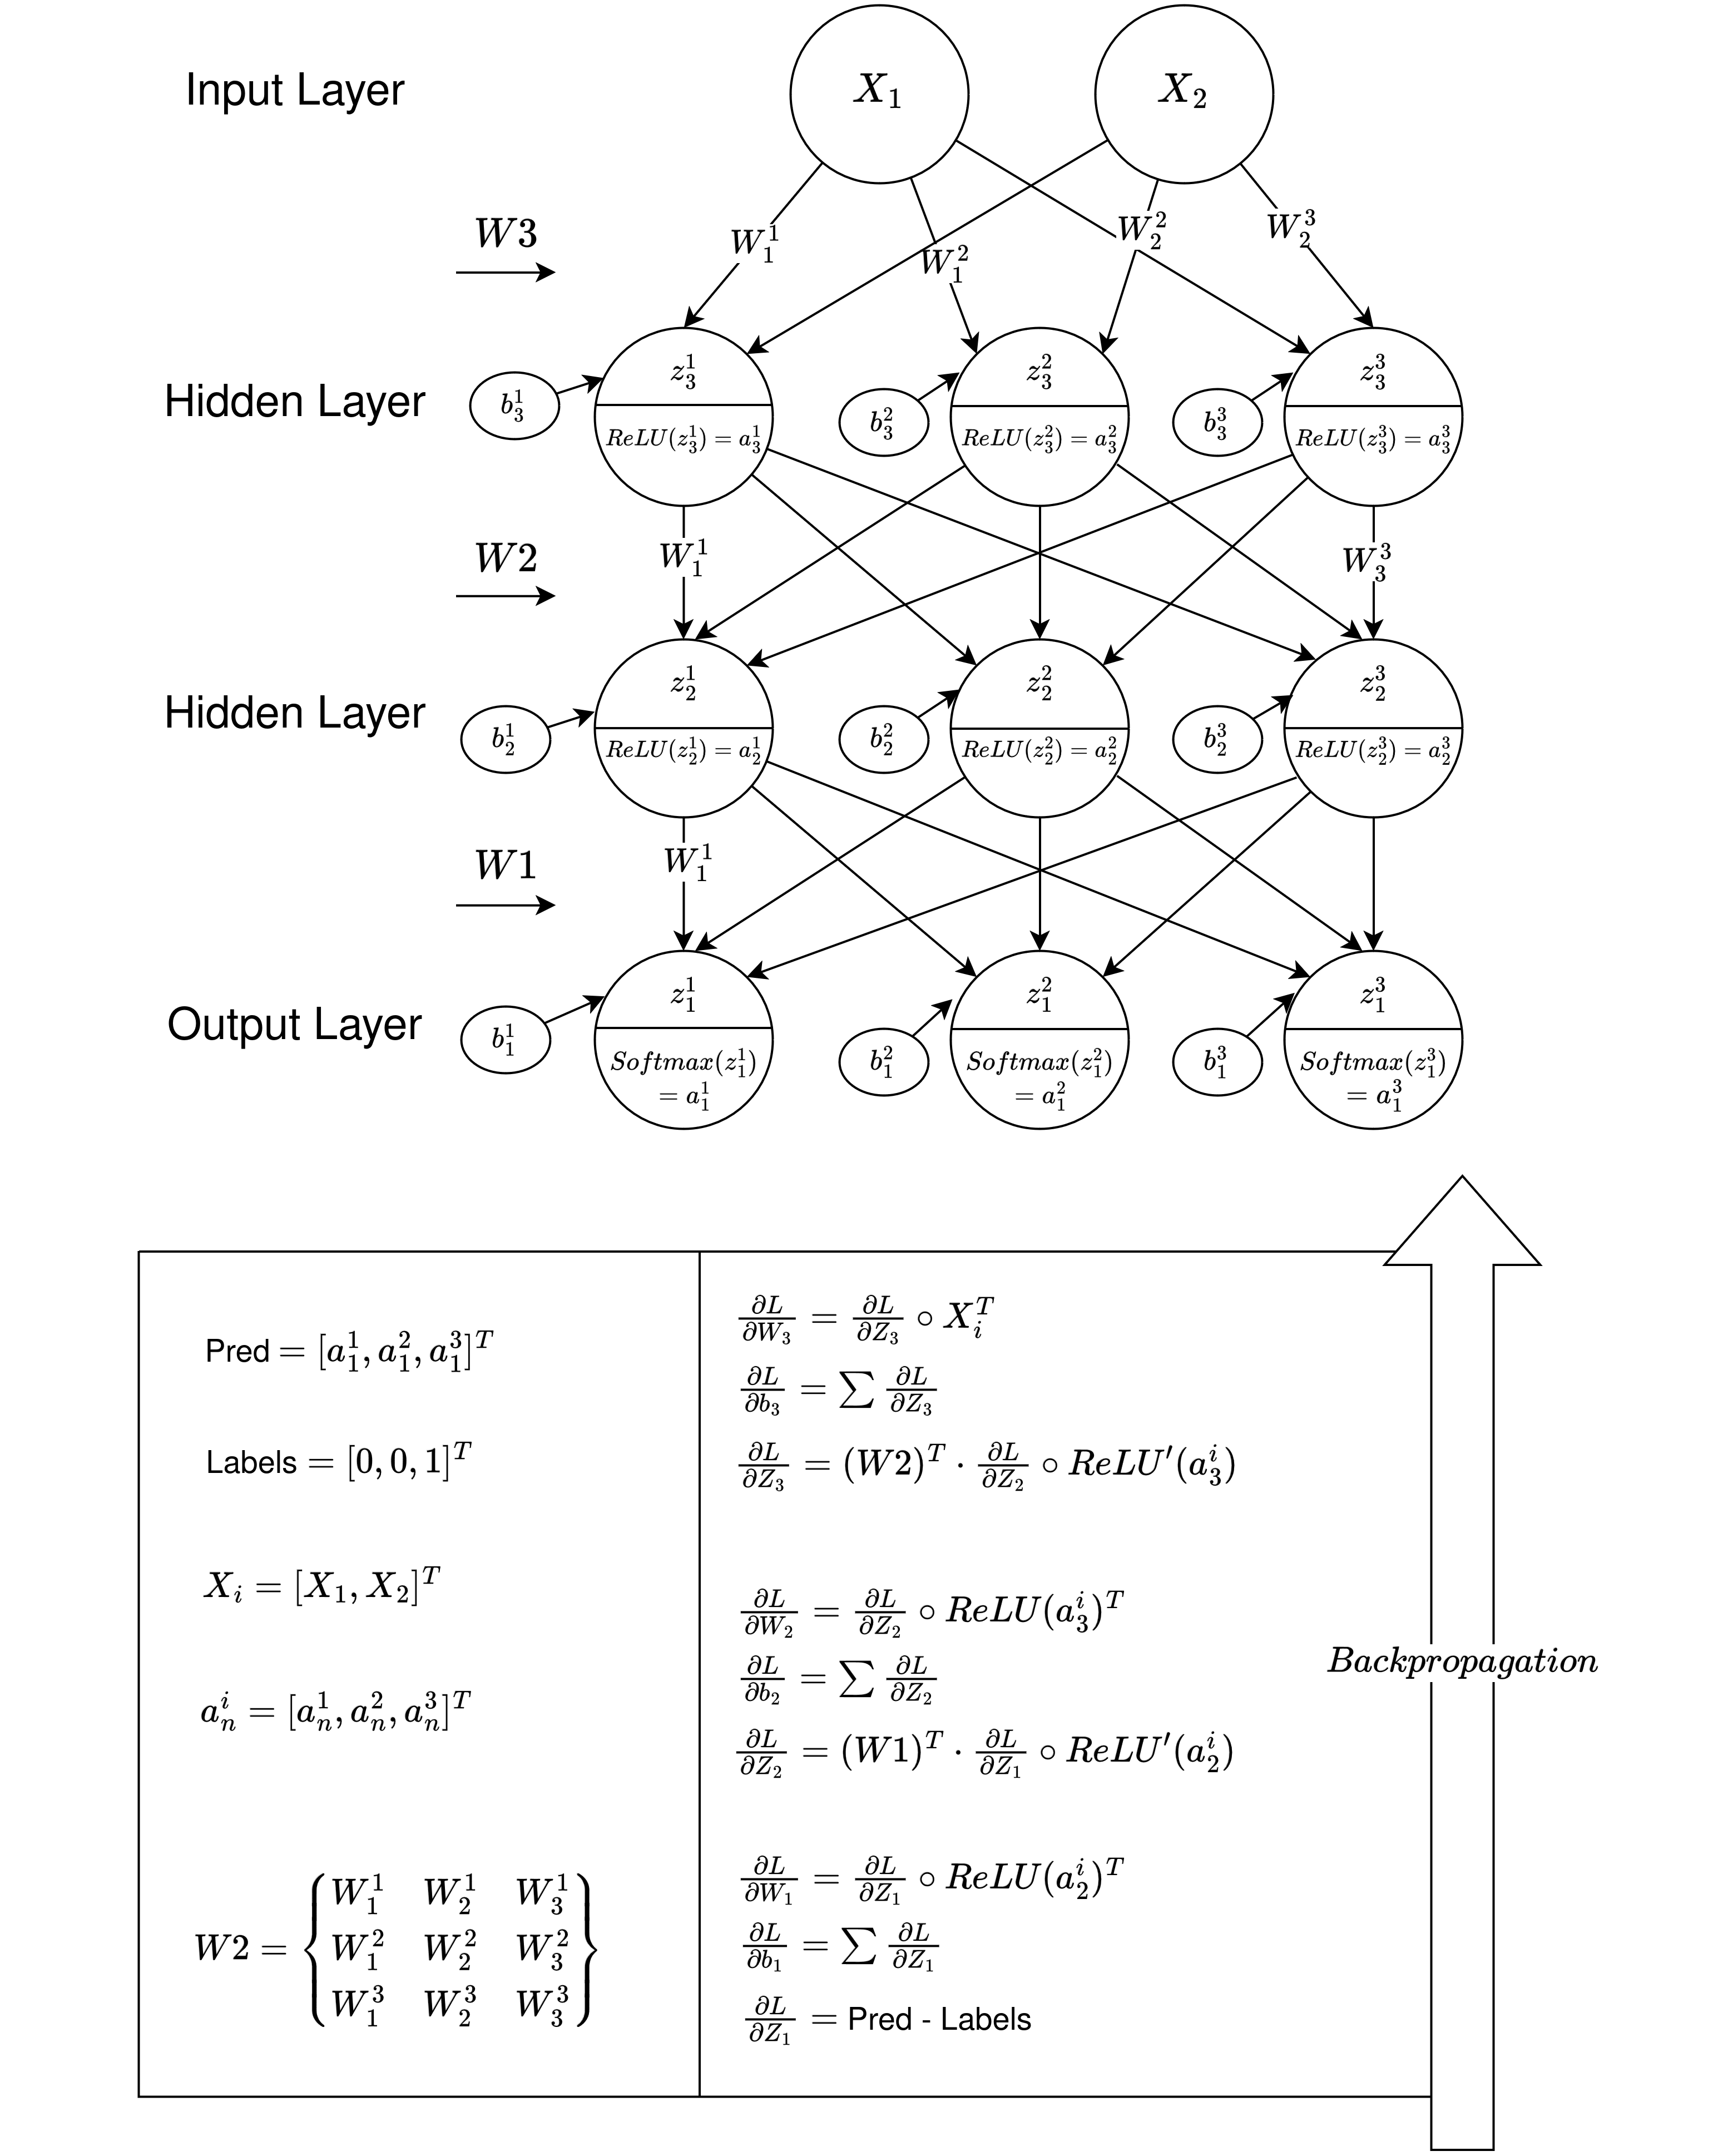
\includegraphics[width=1\linewidth]{template//figures/backpropfigVersionFinal1(1).png}
    \caption{Backpropagation}
    \label{fig:backprop}
\end{figure}

\subsection{Stochastic gradient descent}

Stochastic gradient descent (SGD) is an algorithm to optimize the neural network to minimal loss using forward and backpropagation. Some researchers have suggested that SGD may be the most commonly used algorithm to optimize neural networks (\cite{NIPS2012_6aca9700}). Weights and biases are essentially the values that we want to optimize, so the network output loss is minimized. Most of the deep learning algorithms are based on SGD (\cite{Goodfellow-et-al-2016}), so it can be seen as a fundamental part of deep learning.

The optimization for weight and biases with SGD happens after every sample. A sample is forward propagated through the network to produce predictions. Then the predictions are used to calculate loss and backpropagation is used to find the gradients to weights and biases. These gradients are then used to tune the weights (\(W_{i}\)) and biases: (\(b_{i}\))
\[W_{i} = W_{i} - \alpha \frac{\partial L}{\partial W_{i}}\]
\[b_{i} = b_{i} - \alpha \frac{\partial L}{\partial b_{i}}\]
Here \(\alpha\) is some scalar that we use to define the step size towards the direction defined by the negative gradient. The gradient points in the fastest increasing direction, so by using a negative gradient, these parameters can be adjusted toward the direction that decreases the loss function. By repeating the steps defined above for multiple samples multiple times, we can find the local minima for the loss. By optimizing the weights and biases to perfection, we train the network to produce minimal error with the training data. This leads to a problem called overfitting. Overfitting happens when we get flawless outputs with the training data but can't generalize to unseen data (\cite{overfit}). The goal of the training is to optimize the network to produce correct labels with unlabeled data, so by overfitting, we fail to achieve this goal.

Training data is commonly split into testing and training data (\cite{Goodfellow-et-al-2016}). During the training and splitting the data is shuffled. Test data gives us a portion of the data that we don't use during the training and can be used for testing as unseen data to the network. This helps to identify the overfitting and shows more accurately how the network performs outside the data it has learned from. Additional parameters to the network that are used in training are called hyperparameters. Learning rate or \(\alpha\) is a hyperparameter. The training loop goes through the whole training dataset multiple times during the optimization, "epoch" is a hyperparameter that defines how many times we crawl through the entire training data. Training can also be set to a halt when test data accuracy starts rising while the training data accuracy still decreases, this is considered an early stop (\cite{overfit}). Penalties to the loss function can be set to motivate lesser weights to be used. Other techniques like dropout can be added, more data can be gathered or noise added (\cite{overfit}). Dropout is a technique where random nodes are deleted during the training. Ultimately the optimal hyperparameters and techniques are case-specific but generally avoiding common known problems is helpful. 

Training may be extended, particularly with large deep networks, due to the iterative nature of SGD optimizing parameters after processing each sample. A similar algorithm is batch gradient descent, also known as batch learning. This method uses the entire training data before updating the parameters. The batch method finds the true gradient instead of an estimate as in SGD but is slower and SGD often produces better results (\cite{LECUN2000}). Mini batch gradient descent is a method where training is done via batches. Batch size is an additional hyperparameter that defines the batch size. This method splits the training data in each epoch into a mini-batch consisting of multiple samples that are then all forward propagated through the network simultaneously. Then the backpropagation is done similarly to all the predictions once, and the average gradients are used to update the weights. 


\subsection{Types of neural networks}

Based on the simple neural network many architectures have been built to suit specific domains or problems. They expand or add to the basic idea of neural networks and utilize similar algorithms in training.

Convolutional neural networks (CNN) introduce the concepts of convolution and pooling. CNNs are designed to handle data that has a grid-like topology and are therefore suitable for image-related tasks (\cite{Goodfellow-et-al-2016}). The simplified concepts of pooling and convolution for a 6x6x1 image are illustrated in Figure \ref{CnnExpl}. Values in the kernel are considered learnable weights that are tuned similarly to regular weights connecting neural networks. Multiple kernels can be used in a single convolutional layer, and these layers can be vertically stacked to capture higher dimensional features. Pooling and convolutional layers can be feature extraction layers that eventually are flattened and fed into a regular fully connected neural network that produces the output. Stride defines how much the kernel is moved when it is applied. A 3x3 kernel applied with stride = 1 to 6x6x1 would mean 16 dot products in total. If we had three-channel pictures, for example RGB, a kernel would have the same depth. Pooling layers calculate the maximum or average of the kernel-sized region that is similarly slid over the grid. Additional noise by flipping or zooming the images and padding to the borders are common methods that are applied to CNNs to reduce overfitting. CNNs can significantly reduce the number of parameters in the network compared to FFNNs (\cite{oshea2015introduction}) and capture features of the image effectively. The training follows similar steps and is based on the same fundamental algorithms as described with MLP.

\begin{figure}
    \centering
    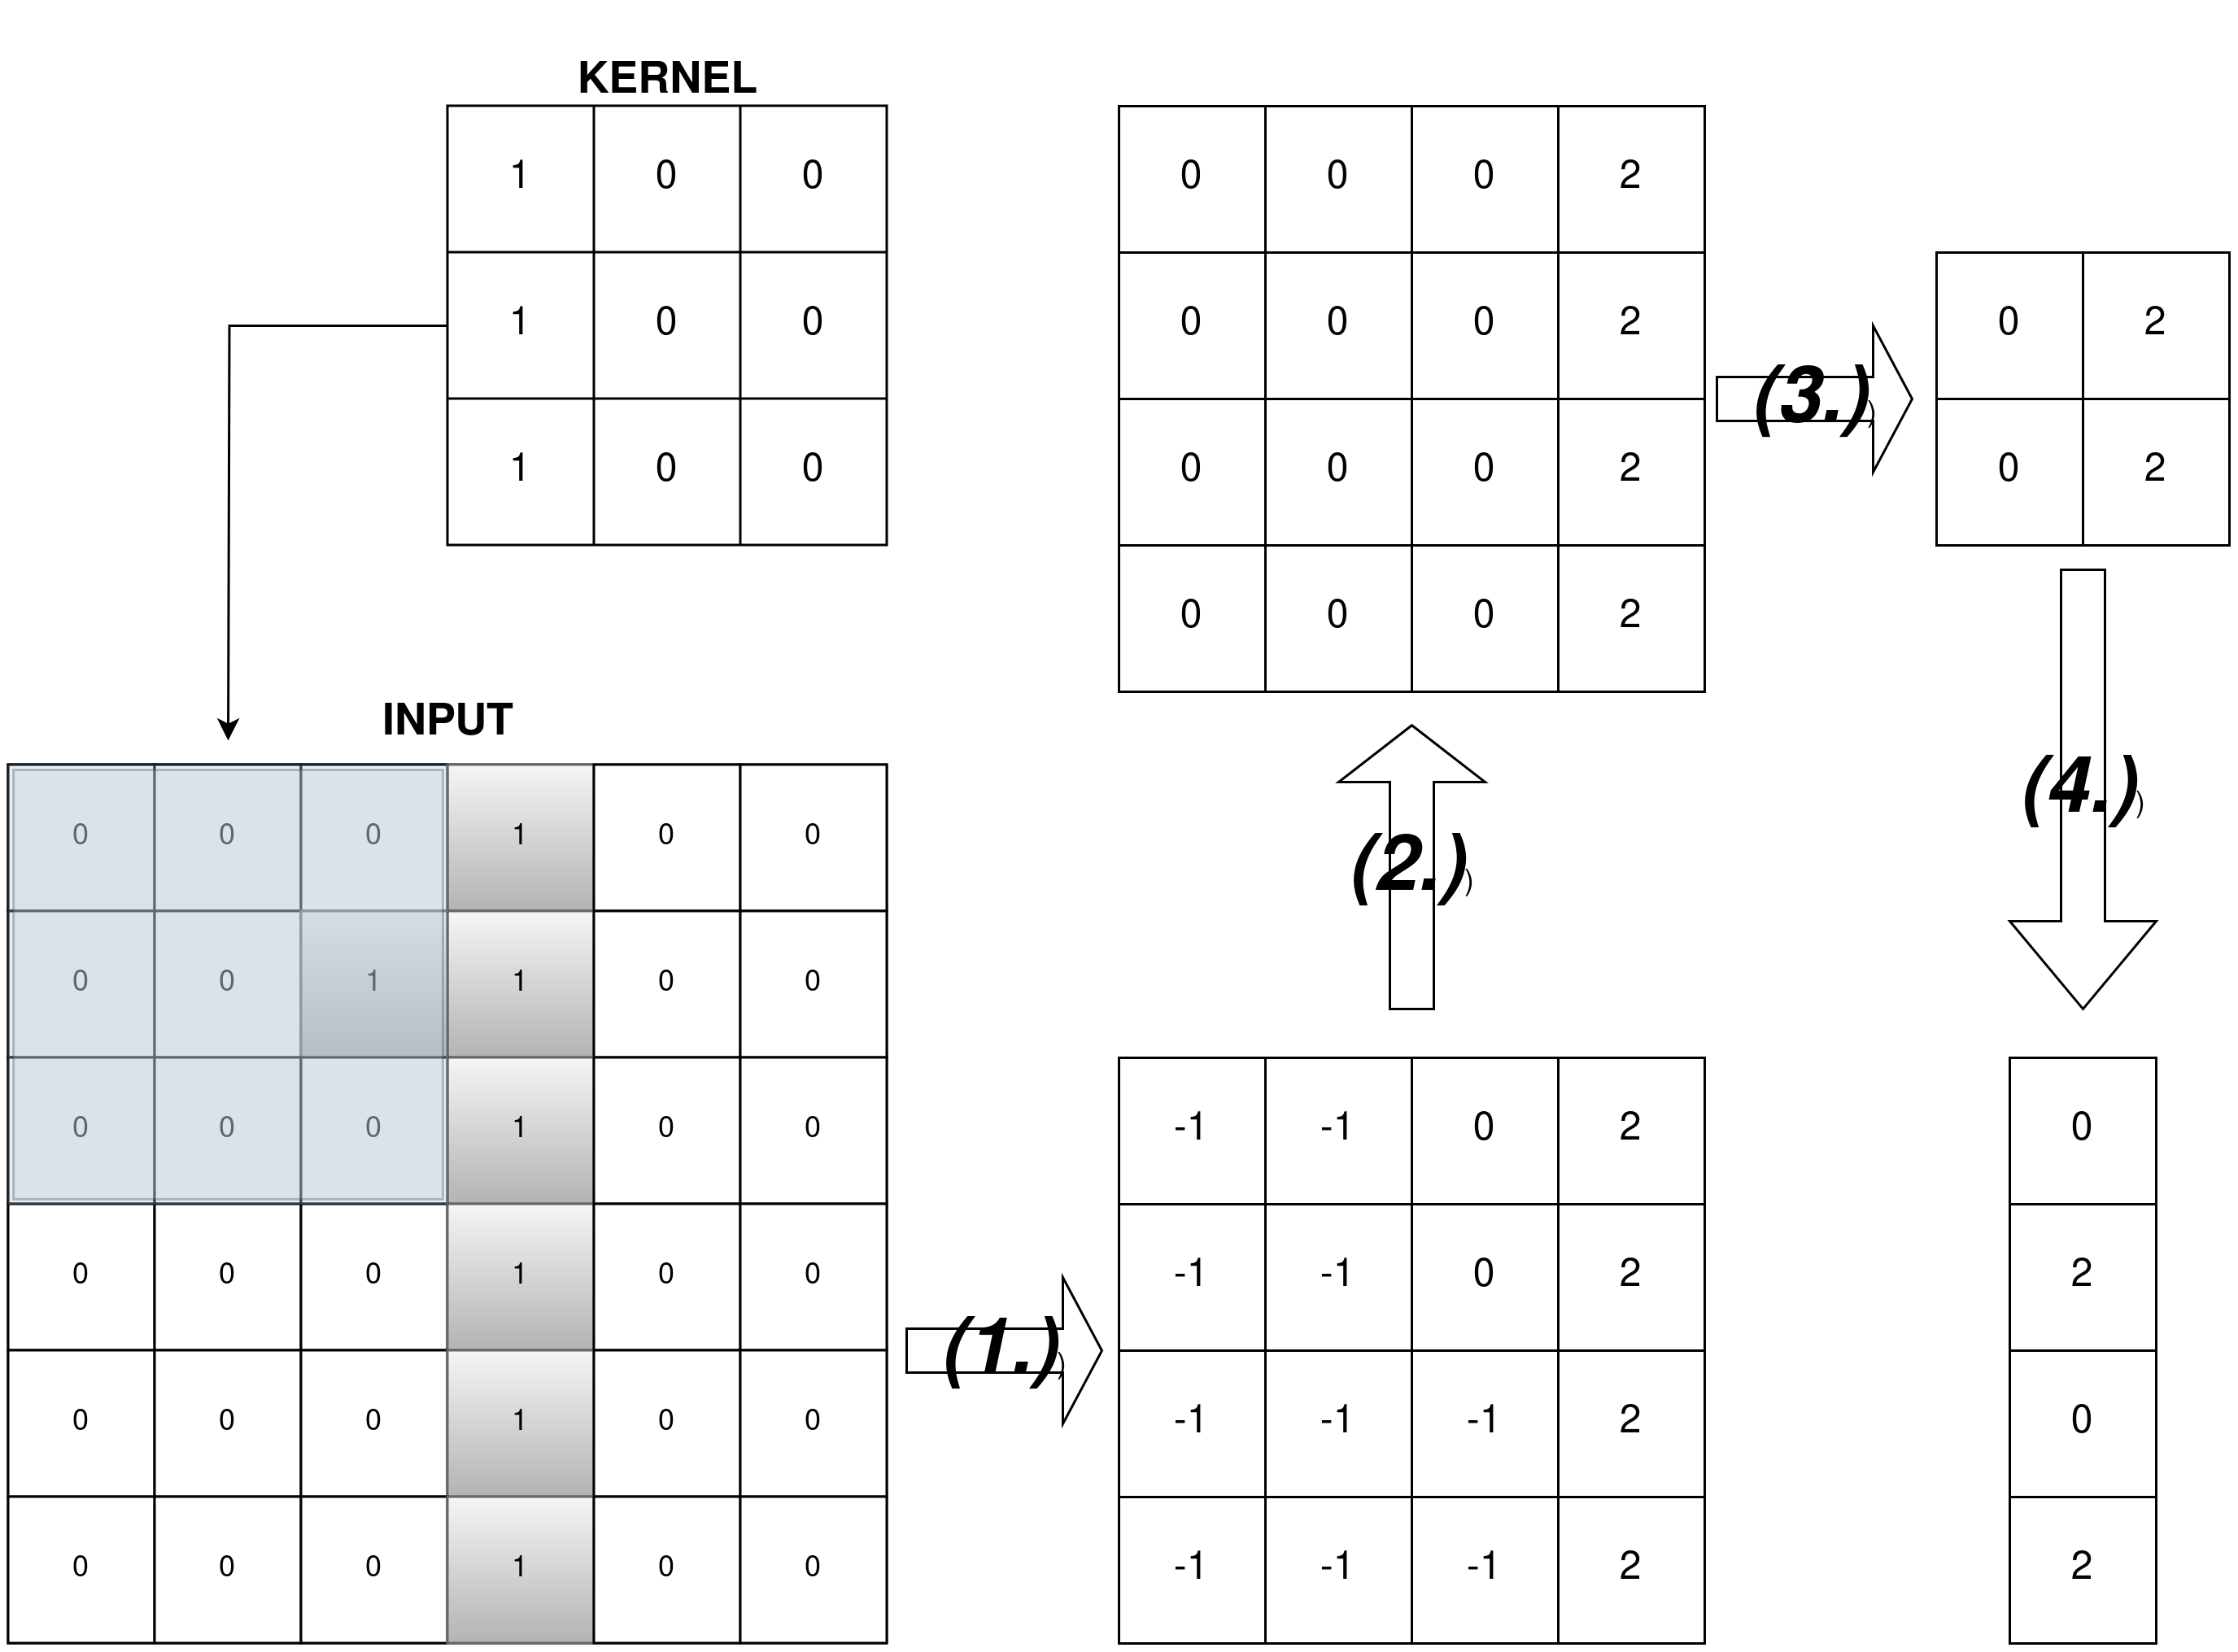
\includegraphics[width=0.75\linewidth]{CNN2EXPL.png}
    \caption{Key concepts of feature extraction layers in CNNs: (1.) Convolution with single 3x3 kernel(stride(1)) and bias[-1], (2.) Elementwise ReLU activation for the 4x4 feature map, (3.) Max-pooling (stride(2)), (4.) Flattening 2x2 to 4x1}
    \label{CnnExpl}
\end{figure}


Recurrent neural networks (RNN) are another commonly known architecture. RNNs are used with sequential data, like stock prices, weather history, or natural language. FFNNs processes all the inputs simultaneously, while RNNs processes sequential data by applying each input in order to the model (\cite{schuster1997bidirectional}). This allows the use of recurrent connections that can carry information from the previous part of the sequence to the next part. Suppose we have a sequence of some signal of integers in sequence \(X = \{ 4_{t1},5_{t2},6_{t3} \}\). The first input would be 4, and the recurrent connection \(M\) set to 0, by feedforwarding this to network, we would then have some updated \(M_1\) that could affect the next input of the sequence. The architecture shares the weight and biases so it can be easily unrolled as the only changing part is the input and the incoming value from the recurrent connection as \(M_i\). The unrolling and vanilla RNN are illustrated in \ref{RNNEXPL}. These blocks can be stacked horizontally to make the network deeper. The unrolling and the shared parameters also allow flexibility on inputs as the blocks can be unrolled according to the input sequence length. The use of activation functions, weights, and biases in the operations and connections behave similarly to the MLP. Training is done similarly with forward propagation, backpropagation, and gradient descent with some modifications to address the recurrent aspects (\cite{biglecun}). Unrolling long sequence inputs shows the main problems in RNNs, vanishing gradients, and the inability to retrain information in the memory (\cite{hochreiter1998vanishing}). Vanishing or exploding gradient is a problem where, during the backpropagation the gradients either vanish or explode, making the optimization difficult.

Long short-term memory network (LSTM) is a modification of RNNs introduced to address the vanishing gradient problem and use the memory aspect more effectively (\cite{LSTMS}). Many modifications built on top of the idea of vanilla RNN:s exist but the LSTM is one of the well-known ones. The LSTMs behave similarly to vanilla RNNs, a single block is illustrated in \ref{RNNEXPL}. LSTM block has 3 gates: forget gate, input gate, and output gate (\cite{LSTMFORGET}). These gates define the amount of memory that is kept from memory and input. Activation functions such as \(Sigmoid\) which maps input to [0,1], and \(Tanh\) that maps the input to [-1,1] are used to scale these gates.  Memory is also known as long-term memory and input as short-term memory. Similarly to vanilla RNN:s, a single block takes inputs sequentially but has 2 recurrent connections coming out of each block. These recurrent connections are not tied up with weights and therefore handle the vanishing gradient problem better.

RNNs can produce multiple and single outputs, and they can also be connected to a regular feedforward network. The main advantage of these architectures is their ability to use previous parts of sequences to influence the next parts with memory. One currently trendy and powerful architecture is a Transformer, introduced by \cite{vaswani2023attention}, which outperforms RNNs in multiple tasks. The Transformer model is built on top of the concepts of RNNs, but the specifics of the new things that this model introduces, such as the attention mechanism, will not be discussed in the scope of this thesis.

\section{Dimensionality reduction methods}

Neural networks and deep learning in general are known to need large amounts of training data. Datasets containing hundreds or more features can be described as high dimensional and are found in multiple domains such as medicine (\cite{dimredbig}). Dimensionality reduction methods aim to reduce the dimensionality and redundancy by mapping the data into a lower dimensionality space. These methods can be used for preprocessing the data in multiple machine learning classification architectures that deal with high dimensional data.

Principal component analysis (PCA) is a well-known linear dimensionality reduction method. PCA finds the lower dimensional representation of the data with the maximum amount of variance explained (\cite{van2009dimensionality}). PCA starts with the normalization of the data and then computes the covariance matrix of the data to find eigenvectors and eigenvalues for each feature. The eigenvalue represents the order of the principal components descending from the largest to the smallest. Eigenvalues also indicate the amount of variance that the component can capture. Eigenvectors can then be used to project the data into the wanted amount of these components. 

Autoencoders (AE) can also be used as dimensionality reduction methods. Autoencoders are FFNNs that aim to learn the input from reduced dimensions. This is done by forcing the data into lower dimensions and reconstructing the input from there. Multiple variations of autoencoders exist, such as multilayer autoencoders (MAE), which are simply networks with more than one hidden layer. Autoencoders hold an odd number of hidden layers and can be described with an encoder and a decoder that have shared weights (\cite{van2009dimensionality}). The bottleneck is the middle layer in the network that captures the lower dimensional representation of the input. An illustration of MAE with six hidden layers, an input layer size of \(6\), and a bottleneck size of \(3\) is found in \ref{MAE}. The encoder can be thought of as the layers before the middle layer in the network that reduces the input data to the bottleneck. The bottleneck is the layer in the middle that holds fewer nodes than there are features in the data, forcing the compression of the data. The decoder is then taught as layers after the bottleneck reconstructing the input from the bottleneck. By training this kind of network we can learn a lower-dimension representation of the data by using the data from the bottleneck layer that is forced to produce it.

\begin{figure}
    \centering
    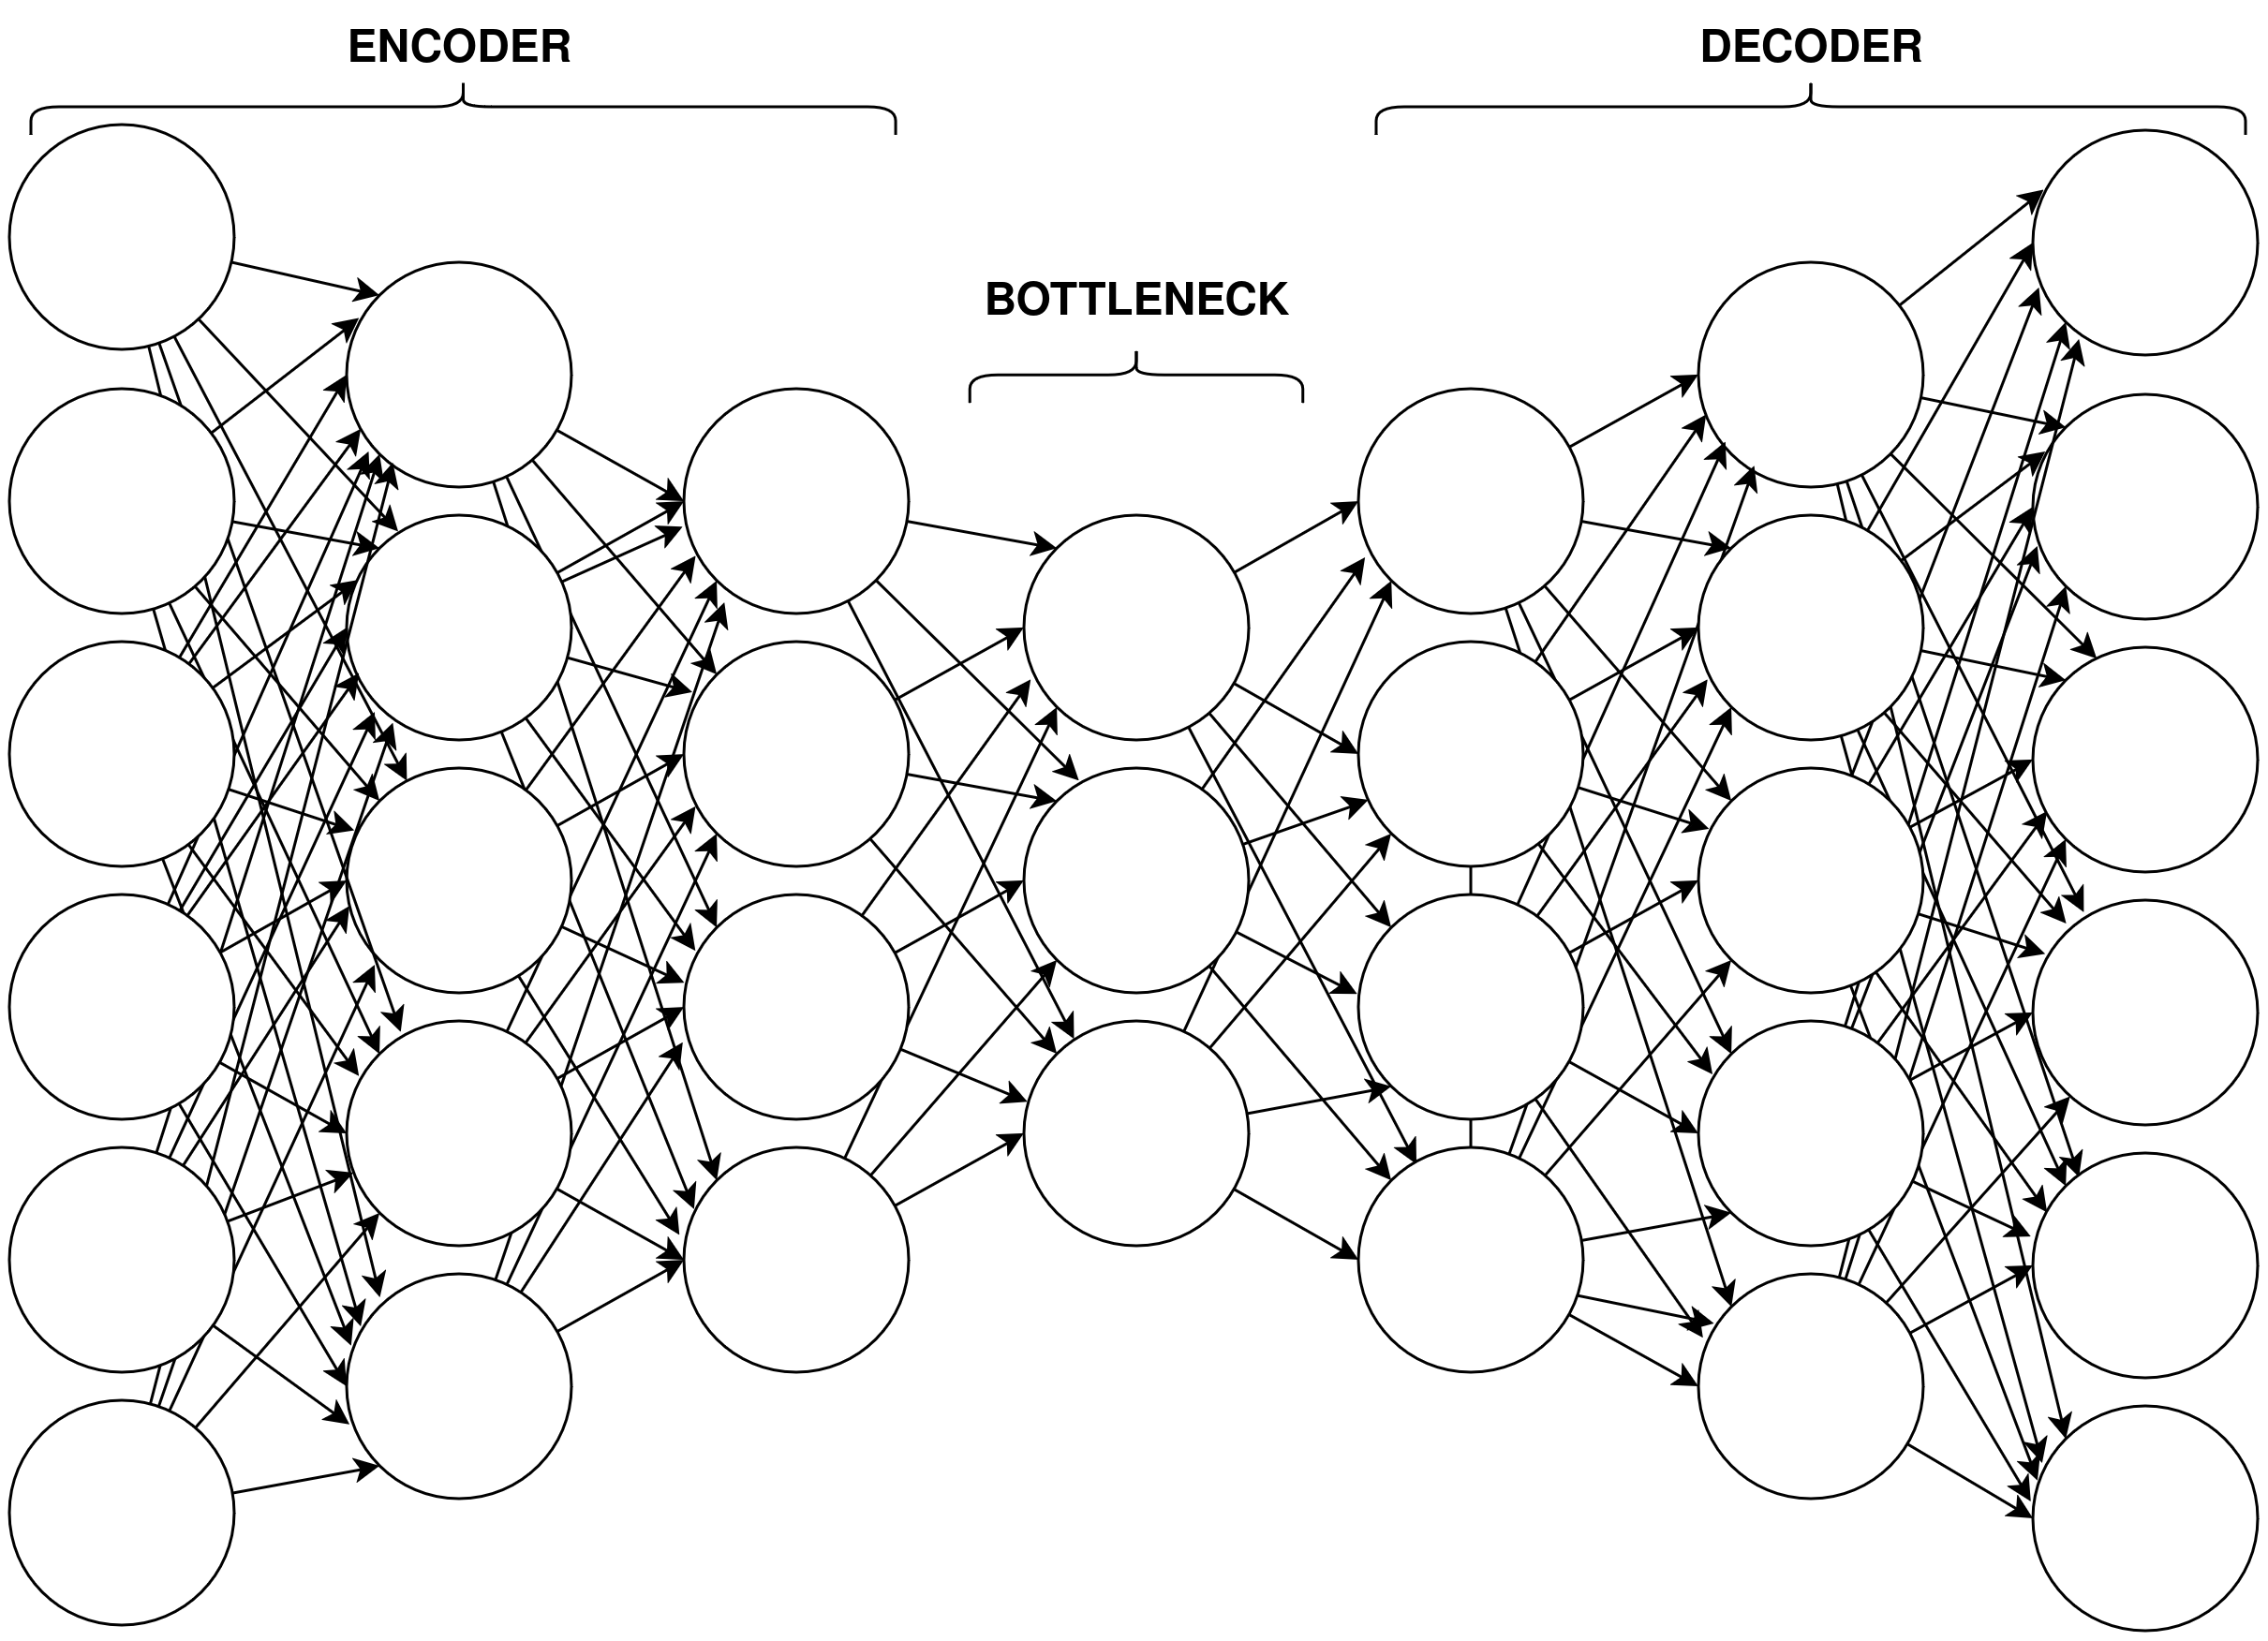
\includegraphics[width=0.75\linewidth]{template//figures/MAE.png}
    \caption{Illustration of the MAE structure}
    \label{MAE}
\end{figure}
\chapter{Multimodal data fusion\label{results}}

The motivation for using multiple modalities is the additional information that could be gained (\cite{8103116}). Different medical imaging methods may give more detailed information when used together, whereas tabular data may give additional information that can't be gathered from images alone. Building a machine learning model to solve a problem with data from multiple modalities eventually leads to an issue of using the different modalities together. Data fusion combines multiple modalities into a single vector or outcome, depending on the approach. One definition of data fusion is the analysis of several data sets such that different data sets can interact and inform each other (\cite{7214350}). Different diseases benefit more from certain approaches to data fusion. For example, fusion approaches that enable cross-modal interactions are essential for certain diseases, whereas others may not benefit as much from such interactions. The nature of the problem and data that is available influences the approach's effectiveness. This chapter aims to provide an overview of the common fusion architectures and difficulties associated with data fusion. Fusion strategies can be used for more than two modalities, but for minimum complexity, the approaches are presented with two modalities. Unimodal models are referred to when classifying with a single modality.

\section{Early, intermediate, and late fusion}


Early fusion is considered when the input modalities are fused into a single representation vector before feeding into the model. Early fusion uses only one model, and the difference compared to unimodal models is the input that is fused. Concatenating is one of the strategies to fuse data within early fusion (\cite{10.1093/bib/bbab569}). Concatenation of \(\vec{x} = [1, 2, 3] \text{ and } \vec{y} = [4, 5, 6],\text{ is }  \vec{x} \oplus \vec{y} = [1, 2, 3, 4, 5, 6].\) Feature extraction can help the fusing but it is seen as preprocessing not as a part of the model. Finding a common subspace for data with varying dimensions and removing correlations between modalities is important for successful early fusion (\cite{8103116}). Early fusion approaches can not propagate loss back to the original input features which is a key difference compared to intermediate fusion methods. Early fusion can utilize any supervised machine learning algorithm. Simplified architecture for an early fusion model is illustrated in \ref{fig:early_late} (a).

Using a separate model for each modality where each model outputs a prediction and combining these predictions to produce the final output is considered as late fusion. Probabilities from the independent model outputs are aggregated to produce the final output. The aggregation method varies based on the modalities and the application, for example, averaging and voting-based approaches can be used (\cite{article22}). Outputs of independent models can also be used as input to another model that makes the final prediction. Late fusion approaches make minimal use of the combined effects of modalities compared to early and intermediate approaches since each prediction is done independently. Simplified architecture for late fusion is illustrated in \ref{fig:early_late} (b).

\begin{figure}
\hfill
\subfigure[Early fusion]{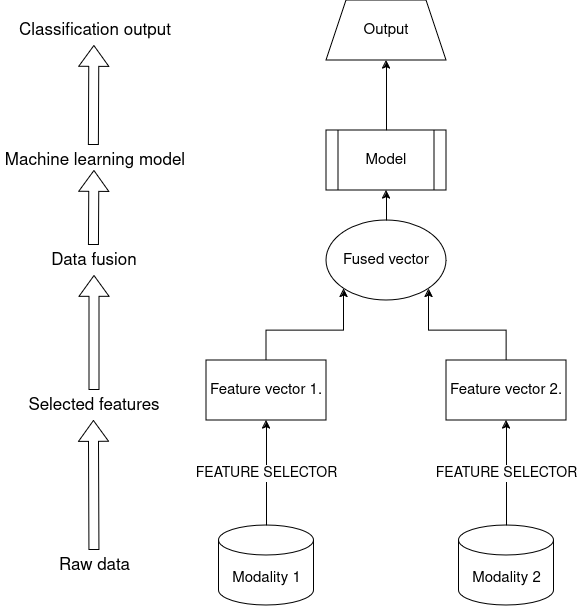
\includegraphics[width=7cm]{template/figures/Early fusion_WHITE.png}}
\hfill
\label{fig:early}
\subfigure[Late fusion]{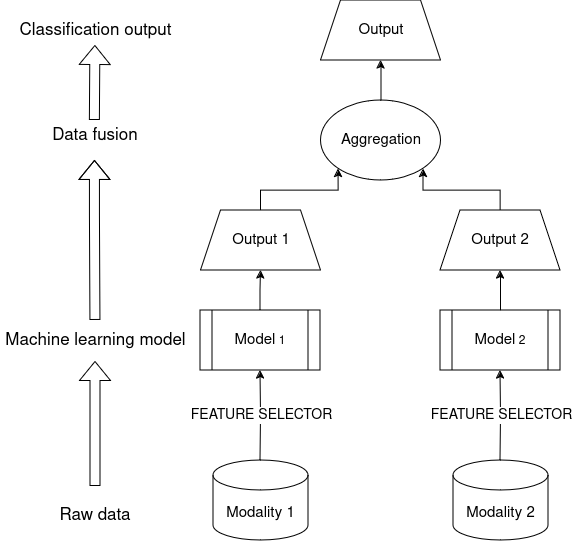
\includegraphics[width=7cm]{template/figures/LateFusion_Fwhite.png}}
\hfill
\label{fig:late}
\caption{Early and late fusion}
\label{fig:early_late}
\end{figure}

Intermediate fusion is an approach where the architecture uses multiple networks together. The model can be separated into multiple unimodal neural networks that towards the end are combined in shared layers. The input to the model is the data from the modalities and the extracted features from independent models are combined into the shared representation layer that in the end produces the output of the model. Figure \ref{fig:intermediate} shows a simplified structure of the intermediate fusion. Fusion between the modalities can also be done in different stages allowing flexibility and PCA or stacked autoencoders can be used to improve the representation in shared layers (\cite{8103116}). Using neural networks in feature extraction and after the fusion allows the loss to be propagated back to the input modality level. This allows better feature extraction since the independent models are also optimized during the training. Intermediate fusion makes use of cross-modal interactions like early fusion and modality-specific models, the same as in late fusion approaches.

\begin{figure}
    \centering
    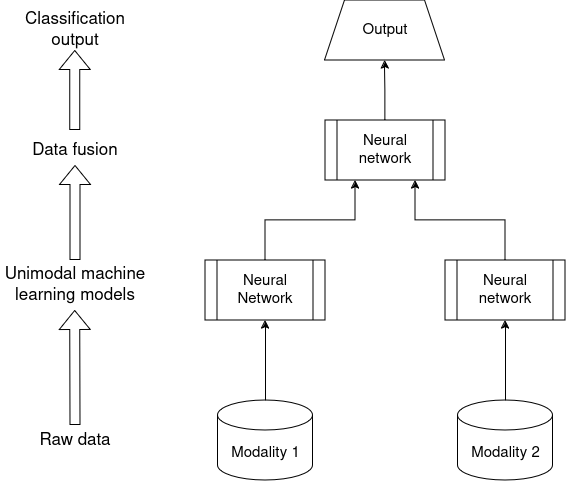
\includegraphics[width=0.5\linewidth]{template//figures/IntermediateFusion_white.png}
    \caption{Intermediate fusion}
    \label{fig:intermediate}
\end{figure}

Early, intermediate, and late fusion can be seen as the baseline for the fusion approaches. While no single approach is proven to be supreme, studies often evaluate and combine different approaches and methods suitable for the given task.
Each of the approaches has advantages and disadvantages. It have been suggested that various unimodal and multimodal approaches should be evaluated when building multimodal models (\cite{article22}), since unimodal models can be used in multimodal approaches and the most suitable fusion approach varies and depends on the problem. Considering the structure of the data fusion approaches, late fusion is suitable in situations where the modalities contain independent aspects of the data. Early fusion can make use of the cross-modal interactions. However, to make use of cross-modal interactions successfully, it might require specific preprocessing techniques. Late fusion architecture can adapt to missing modalities, offering ease when dealing with datasets where data contains different sets of modalities per sample. Independent unimodal models in the late fusion approach also offer easy addition of new modalities as the training can be done only for the additional unimodal models. Early fusion architectures may need retraining of the whole model if new modalities are added. Similarly, when the training is done with data where all modalities are present in each sample, handling missing modalities poses an issue. Relying on one model only reduces complexity compared to models relying on multiple models. Intermediate fusion offers parts from both of these with additional complexity.

Literature review reported that fusion with medical images and clinical data using multimodal fusion generally increased accuracy (1.2–27.7\%) and  Area Under Receiver Operating Characteristic Curve (AUROC\footnotemark{}) of (0.02–0.16) compared to models using a single modality for the same task (\cite{article22}). However, no single fusion strategy performed consistently optimally over all domains. In another review, multimodal data fusion was reported to increase the accuracy over unimodal approaches with a 6.4\% mean improvement in Area Under Curve (AUC\footnotemark[\value{footnote}]) (\cite{articlePreciRev}). The measurements of increased accuracy with multimodal data fusion do not mean that these models would be beneficial for clinical settings and real-world applications. End-to-end applications and prospective studies are needed to validate the relevancy of these models.

\footnotetext{AUC and AUROC are used interchangeably and noted here as they appear in the original paper. More about AUC and AUROC in \ref{appendix:sample}}

\section{Challenges with multimodal machine learning}

Challenges within multimodal machine learning have been outlined as follows (\cite{8269806}):

\textbf{1.} \textit{Representation}: how multiple modalities are meaningfully represented.

\textbf{2.} \textit{Translation}: involves the mapping of data from one modality (A) to another (B).

\textbf{3.} \textit{Alignment}: which parts of one modality directly correspond to another.

\textbf{4.} \textit{Fusion}: how to combine data from multiple modalities, particularly when some data may be missing or certain modalities are more informative than others.

\textbf{5.} \textit{Co-learning}: how to transfer knowledge between different modalities.



All of these are important technical aspects for the successful multimodal machine learning model. It is important to notice that the classification problem itself and the modalities affect heavily the issues that may arise. On top of the five key challenges related to multimodal machine learning and the context-specific ones, traditional problems in machine learning can be similarly found in multimodal architectures. 

\subsection{Explainability}

When machine learning is applied to critical fields such as medicine where the usage might have an impact directly on patient health it is crucial to have explainability on the models (\cite{article44}). Models that use deep learning are often thought of as black boxes and lack explainability. Multimodal machine learning models can have multiple of these employed. Machine learning models and especially deep learning models carry data in abstract representations that might be hard to understand. Similarly, many data fusion methods with feature extractions and shared representations hold data in abstract formats. To understand a decision that is made by the ML model additional metrics or methods can be applied. The eXplainable Artificial Intelligence (XAI) can be seen as a field that aims to produce these methods (\cite{XAI}). An example of this is seen in Shapley values that have been used for measuring the contribution from different modalities (\cite{articlehaim}). Explainability and justification of classification decisions in the models utilized is one of the key challenges to when machine learning models are utilized in medical context. 

\subsection{Data in medical context}

The medical field offers vast amounts of datasets that derive from retrospective studies. Biobanks, national registries, and open-source datasets are sources of data in multimodal medical studies. Datasets such as MIMIC (\cite{articlemimic4}) that are open source are used as a benchmark to compare models. The prospective studies to validate models built with retrospective data are an important part of understanding the true utility and real-world performance of these systems (\cite{kelly2019key}). A specific dataset is needed to apply multimodal machine learning to certain diseases. Privacy in the medical context also limits the data available. In a recent review, small sample sizes and imbalanced samples were reported as common limitations to studies employing multimodal machine learning models (\cite{articlePreciRev}). Small sample sizes and high dimensionality combined increase the sparsity of the data which can also lead to a curse of dimensionality (\cite{articlecurse}). The curse of dimensionality appears in problems like overfitting. While the curse of dimensionality and various problems associated with are well-known in machine learning, assessing them is a necessary step when building multimodal machine learning models. Choosing the correct architecture is an essential part of building a multimodal machine-learning model. Comprehensive evaluation requires the building of multiple models. Conducting high-quality research in this area can be challenging because it involves complex computational models, requires validation studies, and needs expertise from various fields.

\chapter{Applications of multimodal machine learning\label{discussion}}

A recent literature review and highlighted the increased interest in multimodal machine learning (MML) research (\cite{litrewMMLapplic}). In theory, MML approaches can be applied to any domain or problem that links to multiple modalities already solved with machine learning. While the concept of data fusion is not new, deep learning has enabled many possibilities in this field. Particularly within the medical context, data fusion, and MML are a relatively new and currently researched area. Applications of MML appear in recent research papers, but not yet in clinical environments.

\section{Applications in medicine}

\begin{table}[]
\begin{tabular}{lllll}
\hline
                         & Classification task  & Modalities & Fusion approach         &  \\ \hline
Cahan et al., 2023       & PE risk  & 2          & early,late,intermediate &  \\
Venugopalan et al., 2021 & AD, MCI, controls  & 3          & early,late,intermediate                   &  \\
Soenksen et al., 2022    & Multiple & 2-4 (2-11) & early                   &  \\ \hline
\end{tabular}
\end{table}

The medical domain provides many problems that could benefit from MML approach. Biobanks, health centers, registers, and research provide large amounts of different sets of modalities. Literature review ranging from years 2011–2021 of MML in health for diagnosis/prognosis tasks found most papers were from neurology and oncology domains (\cite{articlePreciRev}). Recent Finish article: "The mathematics and statistical models in predicting treatment response in cancer" pointed out, that one of the biggest challenges is the efficient integration of different modalities to achieve the best predictive accuracy (\cite{duodecim}). Biomedical data opens opportunities for a wide amount of other tasks than prognosis and diagnosing. Potential use cases could be in drug discovery, remote monitoring, and many other applications in healthcare (\cite{acosta2022multimodal}). This section focuses on the studies on prognosis and diagnosis as downstream tasks and showcases the use of 2, 3, and 3+ modalities in their respective order. All of these showcased studies are retrospective. It's important to note that usage of machine learning in medical context does not necessarily aim to remove the work of physicians but may help them for example to identify those patients that need specific treatment immediately. Similarly, MML can help to identify the possibility of some diseases earlier. 

\cite{pulmembol} applied MML methods to predict the risk stratification of pulmonary embolism (PE). Evaluation and comparison were done by building multiple models with different fusion strategies in this retrospective study. Three encoders were built to be used as encoders in multimodal settings and as unimodal baseline models for image and EHR modalities. Previously, \cite{pulm1st} introduced CNN-based Stacked Attention Network (SANet), which was used as the main imaging encoder, but also compared to the second baseline image encoder, Swin UNETR Transformer (\cite{SWIN}), in intermediate fusion architectures. Futhermore, TabNet (\cite{arik2020tabnet}), a neural network architecture for tabular data was used as a baseline encoder for EHR modality. For downstream tasks, XGBoost or TabNet was used. Additionally, for early and intermediate fusion architectures, dimensionality reduction methods were evaluated for the fusion layer after concatenation. The bilinear attention network (BAN) (\cite{kim2018bilinear}) was chosen as an additional layer to further enhance the fusion. The best-performing architecture was an intermediate fusion with SANet and TabNet encoders followed by concatenation and BAN for the fusion layer before the last TabNet as a downstream classifier. This architecture significantly increased AUC over the unimodal baseline models showing the possible value gained by using multimodal architecture. Identifying PE early and proper treatment can decrease the deaths caused by this disease (\cite{pulmembol}).


\cite{alzmulti} presented MML approach to classify Alzheimer’s disease (AD), mild cognitive disorders (MCI), and controls. Imaging (MRI), genetic (SNP), and clinical (EHR) modalities were used and evaluated in different combinations. The Alzheimer’s Disease Neuroimaging Initiative (ADNI) (\cite{ADNI}) was used as a data source for this study. The backbone of the Deep MML architecture was built using feature extraction for each modality. MRI features extracted with 3D CNN. SNP and EHR data features were similarly extracted with stacked denoising auto-encoders. Each of these models was trained independently. Extracted features are then used as input after concatenation for the classifier layer making it an early fusion approach. Other deep fusion approaches were not evaluated. K-nearest neighbors (kNN), support vector machines (SVM), random forests, and decision trees were compared as downstream classifiers. This model was compared to shallow models with early and late fusion approaches. Both shallow models employed decision trees and the late version used majority voting. A comparison between models using single modalities was done to highlight the performance of deep models over shallow ones. Deep unimodal approaches outperformed kNN, decision trees, random forests, and SVM approaches with SNP and MRI modalities. Decision trees and random forests achieved similar performance with deep approaches in EHR modality. Similarly, the two shallow models were compared to deep models with kNN, SVM, decision trees, and random forests as downstream classifiers in all possible combinations of modalities. All deep approaches performed better compared to shallow models in every combination of modalities excluding the MRI + SNP. This was explained with small sample sizes. This study demonstrated the possible benefits that can be gained with deep fusion approaches. Similar findings were found in review which stated that leveraging deep learning fusion consistently showed improvements in performance for Alzheimer's disease diagnosis (\cite{article22}). Identifying the AD or MCI early would be beneficial for patients and society as the costs decrease and the progression slowed (\cite{rasmussen2019alzheimer}).


\cite{articlehaim} introduced and evaluated a unified holistic AI in medicine (HAIM) framework. HAIM is built to handle nonfixed-size sets of modalities. Each modality is handled independently with feature extraction models that generate a set of embeddings that can then be used for multiple downstream tasks. This architecture can be modified with any set of modalities and feature extraction models to whatever state-of-the-art models are available. This is seen as early fusion architecture where the machine learning models act as feature extractors. The evaluation of the proposed framework was done with open-source data from MIMIC-IV (\cite{articlemimic4}) and MIMIC-CXR-JPG (\cite{mimicXR}). Images, tabular data, natural language, and time series were used as modalities with 11 sources. For images pre-trained Densenet121 (\cite{densenet}) was used as a feature extractor, similarly for natural language pre-trained Clinical BERT (\cite{bertclinic}) was used. The tasks for evaluation included 10 different chest diagnoses, length-of-stay, and 48h-mortality. XGBoost was used as the final classifier for all of these downstream tasks. Shapley values were reported to analyze the benefits gained from different modalities and models with different combinations of data sources and modalities compared to single-source models. Vision data was found to contribute most to performance in chest diagnostic tasks, while length-of-stay and 48-hour mortality time-series were identified as the most relevant modalities. Multimodal approaches consistently outperformed the single-source models in AUROC with an average improvement of 9-28\% across all downstream tasks. 


\section{Applications in other fields}

Multimodal machine learning can be found in a wide variety of applications and research from multimedia, robotics, and human-computer interaction (\cite{liang2023foundations}). While each field approaches problems from a different angle, the solution can benefit many. Autonomous vehicles could benefit from using multiple modalities but must also handle the data quickly in real-time. \cite{prakash2021multi} introduced a model called TransFuser that utilizes multiple fusion layers between convolutional layers in feature extractors for LiDAR and front-facing cameras. Interestingly the latest versions of widely popular large language models are introduced as multimodal models as they can out and input multiple modalities (\cite{openai2024gpt4} \cite{geminiteam2023gemini}). 


\chapter{Conclusions\label{conclusions}}

In this thesis, we have identified some of the fundamental concepts related to multimodal machine learning and deep learning. We have clarified the differences and identified the common approaches to data fusion. Furthermore, the challenges related to data fusion are presented with a focus on medical diagnosis. Recent studies show the utilization of different data fusion approaches combined with varying machine learning methods. In general, the research questions set for this thesis are answered, as we successfully described the basic problems and methods related to the large and still evolving field of multimodal machine learning in medicine.

Multimodal machine learning has shown potential in medical diagnosing tasks. While many problems remain unsolved, potential benefits have been demonstrated in many retrospective original studies and comprehensive reviews. Research on data fusion and multimodal aspects is expected to continue, and prospective interdisciplinary studies, that allow comparison between similar approaches are needed to validate current findings. Synthetic Data and Explainable Artificial Intelligence could provide important aspects for development and research in this field. In the medical context, research on unimodal models is also important as models that improve on a single modality can then be utilized in MML architectures. Recent advances in deep learning methods such as Transformer architecture might also provide additional tools for data fusion. 


\chapter*{The use of artificial intelligence in the thesis}

\textit{Research rabbit}  was used to find papers relevant to the topic \href{https://www.researchrabbit.ai/}{-Link}

\textit{Grammarly} was used for spelling and grammar corrections \href{https://www.grammarly.com/}{-Link}

%%%%%%%%%%%%%%%%%%%%%%%%%%%%%%%%%%%%%%%%%%%%%%%%%%%%%%%%%
%\cleardoublepage                          %fixes the position of bibliography in bookmarks
%\phantomsection
\addcontentsline{toc}{chapter}{\bibname}  % This lines adds the bibliography to the ToC
\printbibliography

%%%%%%%%%%%%%%%%%%%%%%%%%%%%%%%%%%%%%%%%%%%%%%%%%%%%%%%%%
\backmatter
\begin{appendices}

%% A sample Appendix

\appendix{Additional figures\label{appendix:sample}}
Area Under the Curve (AUC) measures the accuracy or performance of the model with different thresholds. To calculate ROC and area under curve (AUC) we need a True positive rate (TPR) and a False negative rate (FPR). 

\(TPR = \frac{TruePositive}{TruePositive + FalseNegative}\)
\(FPR = \frac{FalsePositive}{FalsePositive + TrueNegative}\)


\begin{table}[h]
\begin{tabular}{ll|ll|}
\cline{3-4}
 &  & \multicolumn{2}{l|}{Actual}              \\ \cline{3-4} 
 &  & \multicolumn{1}{l|}{Positive} & Negative \\ \hline
\multicolumn{1}{|l|}{\multirow{2}{*}{Predicted}} & Positive & \multicolumn{1}{l|}{True Positive}  & False Positive \\ \cline{2-4} 
\multicolumn{1}{|l|}{}                           & Negative & \multicolumn{1}{l|}{False Negative} & True Negative  \\ \hline
\end{tabular}
\end{table}

\begin{figure}[h]
    \centering
    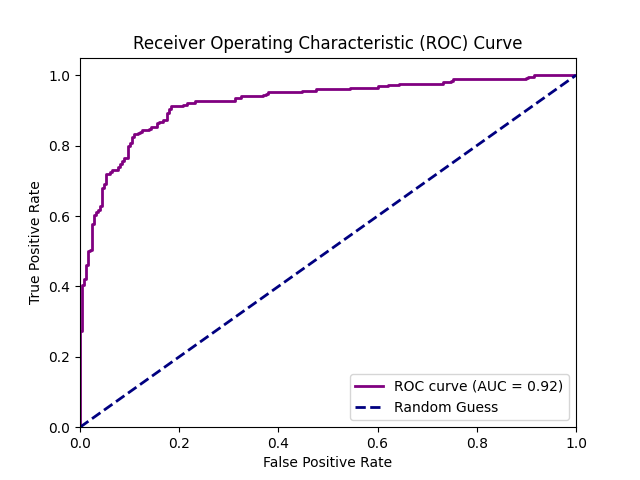
\includegraphics[width=1\linewidth]{template//figures/roc_curve_example1.png}
    \caption{AUC and ROC example}
    \label{fig:enter-label}
\end{figure}




\begin{figure}[h]
    \centering
    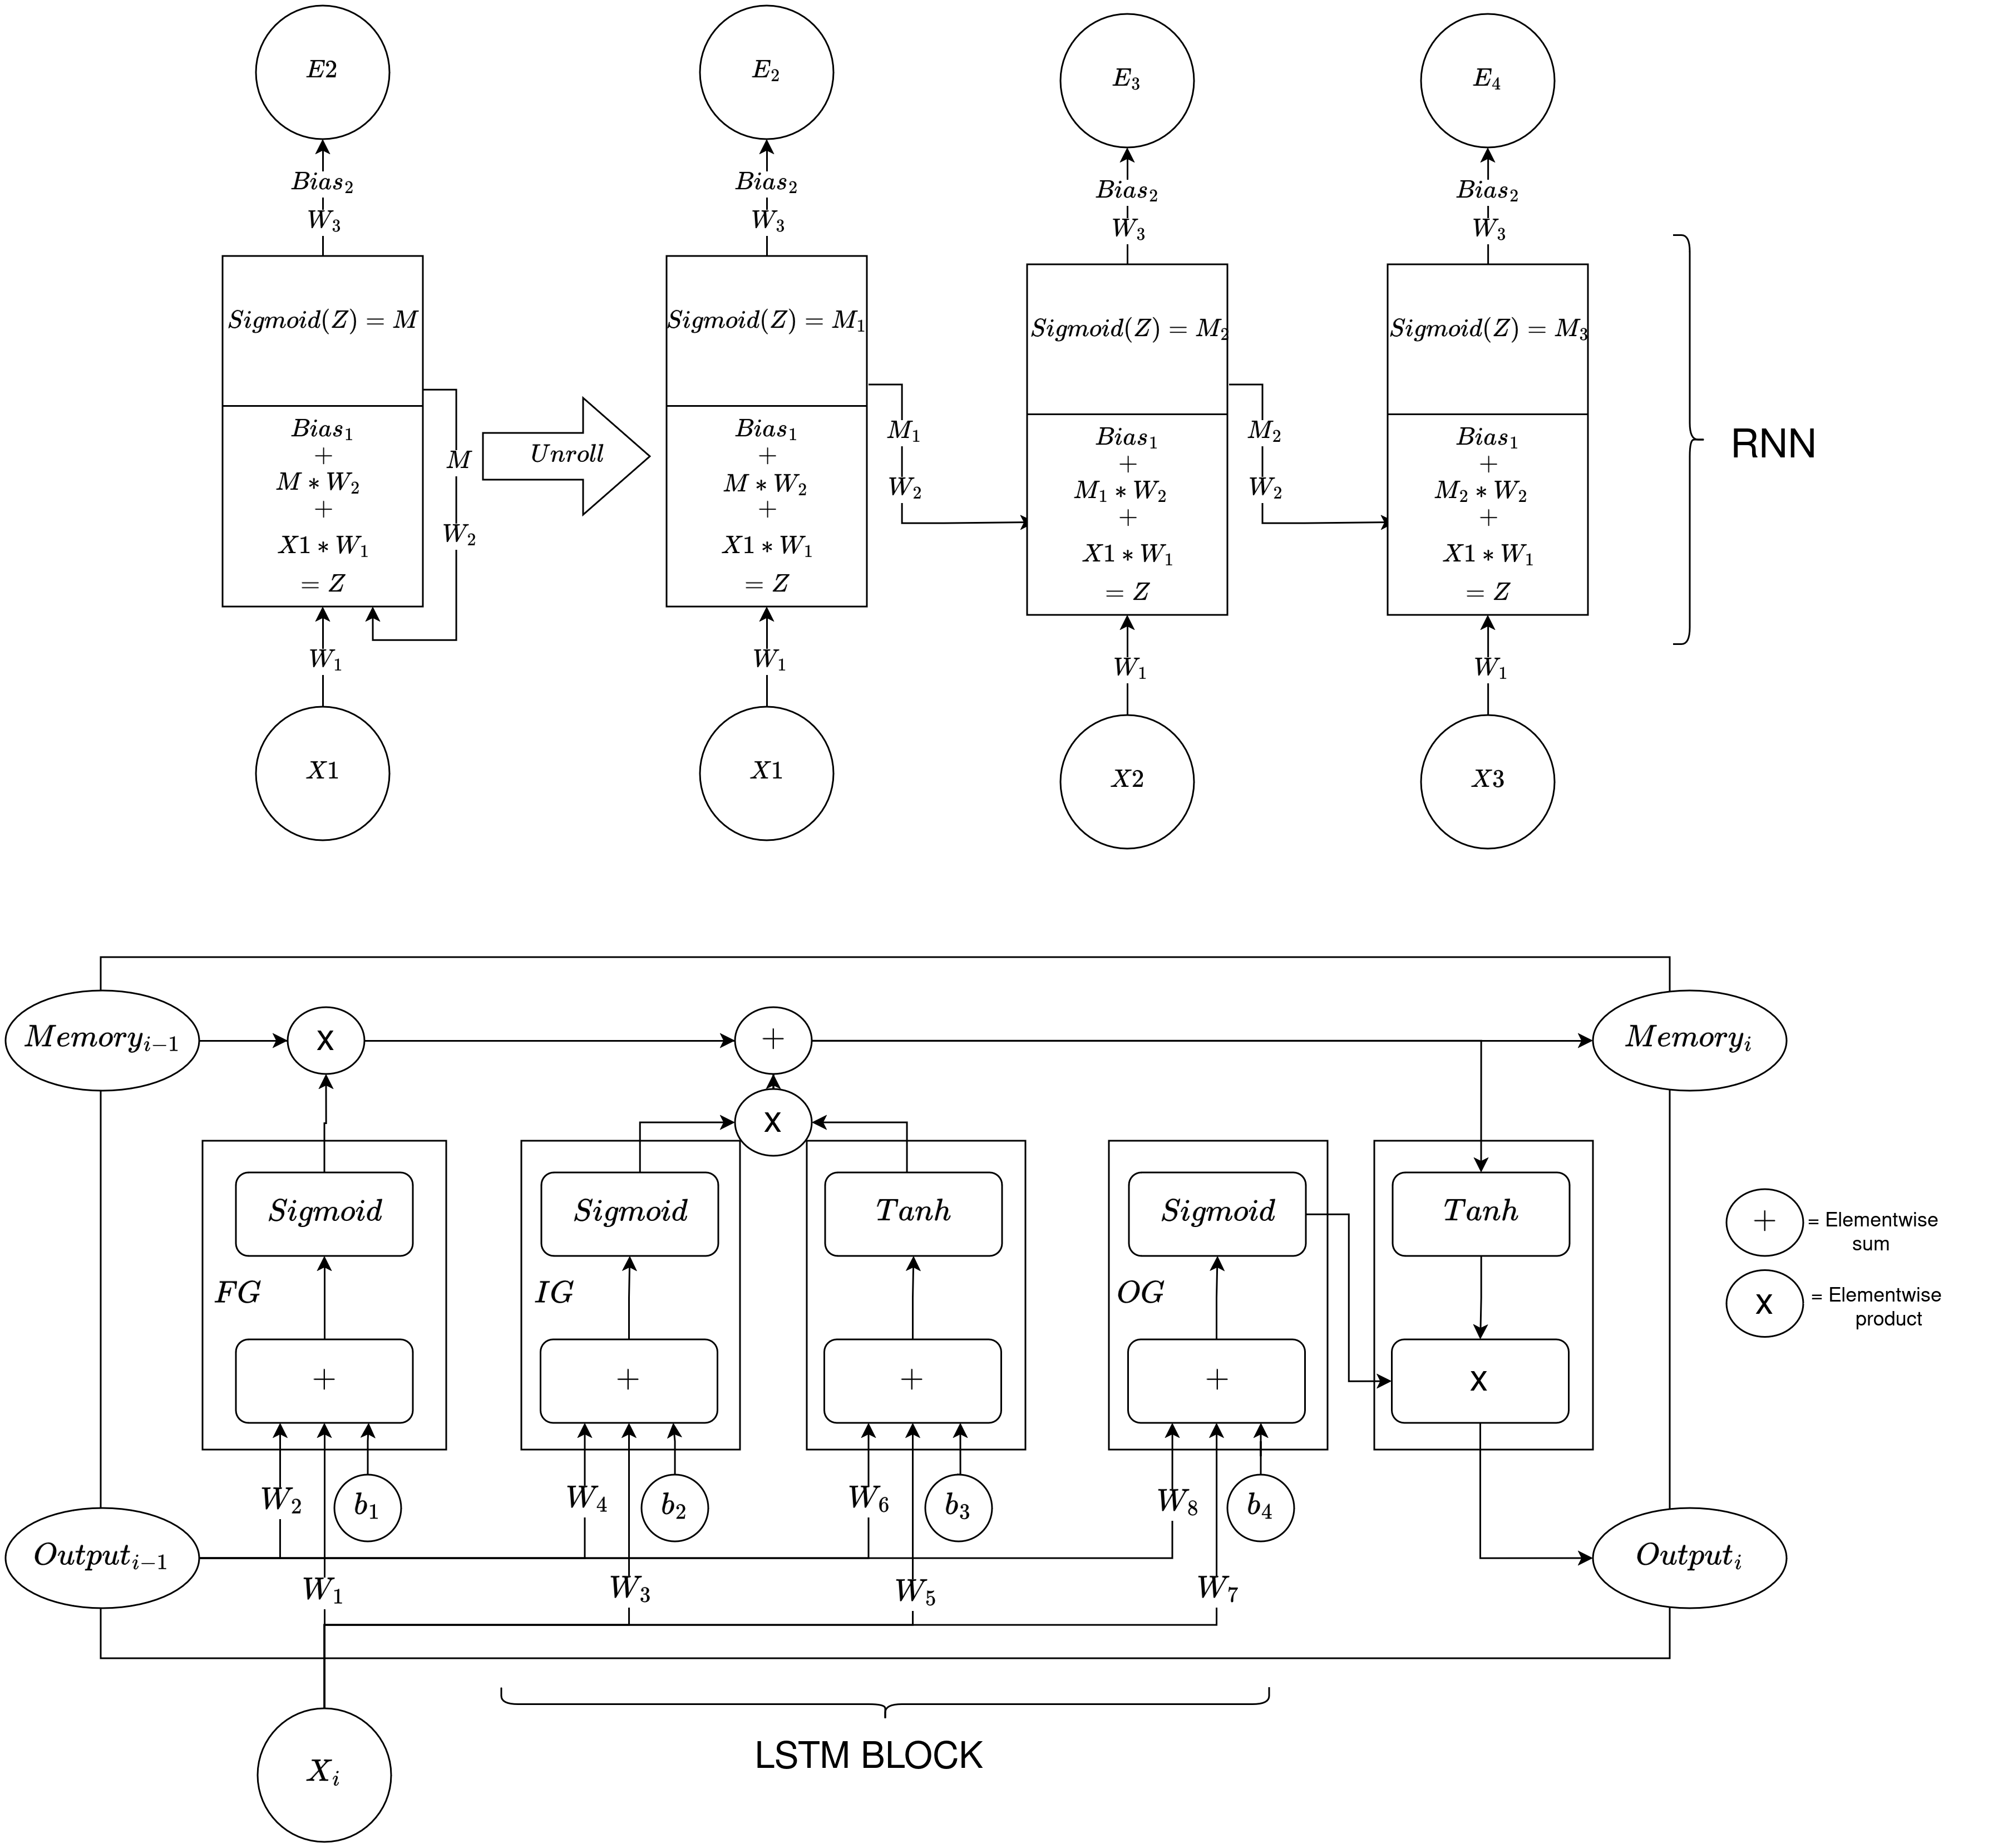
\includegraphics[width=1\linewidth]{template//figures/RNNEXPL_R.png}
    \caption{Sturcture of RNN and LSTM illustrated [inspired: (\cite{googleblog})]}
    \label{RNNEXPL}
\end{figure}


%% another appendix
%
\appendix{Instructions for LaTex}

\section{General Setup}

In the HY-CS-main.tex file you will find the following STEPS 0--5. Below you can find related instructions.
\vspace{0.5cm}

\textbf{STEP 0 -- Access the thesis template}

\begin{itemize}
\item Import the thesis template into a new Overleaf project. The easiest way to do it is to:
\begin{itemize}
    \item Obtain a zip file of the LaTeX template from the webpage of your programme.
    \item Go to \url{https://www.overleaf.com/edu/helsinki} and login to Overleaf with your university credentials.
    \item Go to the list of your projects at \url{https://www.overleaf.com/project}, click ``New Project'' and ``Upload Project''.,  the projects under your account 
    \item Then upload the zip with the template.
    \item You are now ready to write your thesis in Overleaf by editing the template, you can start by renaming the project.
\end{itemize}
\end{itemize}


{\textbf{STEP 1 -- BSc or MSc thesis?}}
\begin{enumerate}
\item Select whether your are writing BSc (tkt) or MSc (csm for CS) thesis.
\item Select your language: \texttt{finnish}, \texttt{english}, or \texttt{swedish}.
\item If you are writing MSc select your line / track.
\end{enumerate}


{\textbf{STEP 2 -- Set up your personal information}}

\begin{enumerate}
\item Specify the title of your thesis with \texttt{\textbackslash title\{\}}.
\item Specify your name to the author field with \texttt{\textbackslash author\{\}}.
\item Specify the names of your supervisors of the thesis with \texttt{\textbackslash supervisors\{\}}.
\item Specify the keywords of the thesis with \texttt{\textbackslash keywords\{\}}.
\item Specify the ACM classification terms of the thesis with \texttt{\textbackslash classification\{\}}. See \url{https://dl.acm.org/ccs} for more information.
\end{enumerate}

{\textbf{STEP 3 -- Write your abstract}}

\begin{itemize}
\item You can have the abstract in multiple languages with the \texttt{otherlanguages} environment. The example below shows how to provide an English abstract: 

\begin{verbatim}
\begin{otherlanguage}{english} 
\begin{abstract}
Your abstract text goes here. 
\end{abstract} 
\end{otherlanguage}
\end{verbatim}

\end{itemize}

{\textbf{STEP 4 -- Writing your thesis}}

\begin{enumerate}
\item There are some minimal contents and instructions below 
\item Remove, or comment out, this appendix from your thesis.
\end{enumerate}

{\textbf{STEP 5 -- Set your bibliography style}}

\begin{itemize}
\item The default is Author-Year style (Einstein, 1905), but it can be easily changed to numbered [1] or alphabetical [Ein05] , as the examples of these are in comments.
\item Discuss the style to use with your supervisor.
\end{itemize}

\section{Bibliography in Latex}

The bibliography is defined in a separate \texttt{.bib} file. For this template, it is named \texttt{bibliography.bib} and includes the content show in Figure~\ref{bibexamples}.

Chapter Bibliography lists all the works that you refer to in your text. You refer to the works in the bibliography using an appropriate \emph{citation key}.
%
%This thesis template contains an example of a bibliography.


References are done using \texttt{\textbackslash citep\{einstein\}}, which generates in text a citation formatted according to the selected style \citep{einstein}, or \texttt{\textbackslash citep\{latexcompanion,knuth99\}}, which generates \citep{latexcompanion,knuth99}. 
As examples of a different kinds of citations (see how these look in the Latex source), we can write \citep{einstein} to refer to the work written by \citeauthor{einstein} in \citeyear{einstein}, because the work by \citet{einstein} appears in the bilbliography included in this template.

Note that there are different possible styles for the bibliography and citation keys.
%
Consult your supervisors on the chosen style -- and once you arrive at a preferred style, use it consistently throughout the thesis.

\begin{figure}[ht]
    \centering
    \begin{scriptsize}
\begin{verbatim}
@article{einstein,
    author =       "Albert Einstein",
    title =        "{Zur Elektrodynamik bewegter K{\"o}rper}. ({German})
        [{On} the electrodynamics of moving bodies]",
    journal =      "Annalen der Physik",
    volume =       "322",
    number =       "10",
    pages =        "891--921",
    year =         "1905",
    DOI =          "http://dx.doi.org/10.1002/andp.19053221004"
}
 
@book{latexcompanion,
    author    = "Michel Goossens and Frank Mittelbach and Alexander Samarin",
    title     = "The \LaTeX\ Companion",
    year      = "1993",
    publisher = "Addison-Wesley",
    address   = "Reading, Massachusetts"
}

@book{knuth99,
    author    = "Donald E. Knuth",
    title     = "Digital Typography",
    year      = "1999",
    publisher = "The Center for the Study of Language and Information",
    series    = "CLSI Lecture Notes (78)"
}\end{verbatim}
\end{scriptsize}
    \caption{Examples of bibliographic reference in .bib file.}
    \label{bibexamples}
\end{figure}

%In the last reference url field the code \verb+%7E+ will translate into \verb+~+ once clicked in the final pdf.

\section{Some instructions about writing in Latex}

The following gives some superficial instructions for using this template for a Master's thesis. For guidelines on thesis writing you can consult various sources, such as university courses on scientific writing or your supervisors.

For more detailed instructions, just google, e.g., "Overleaf table positioning", and your chances of finding good info are pretty good.  


\section{Figures}
Besides text, here are simple examples how you can add figures and tables in your thesis.
Remember always to refer to each figure in the main text and provide them with a descriptive caption.

Figure~\ref{fig:logo} is an example of a figure in the document (see the source about how to add them). 
%Using figures is particularly useful to display plots of experimental results.

\begin{figure}[ht] 
\begin{center}

\includegraphics[width=0.3\textwidth]{template/figures/HY-logo-ml.png}
\caption{University of Helsinki flame-logo for Faculty of Science.\label{fig:logo}}
\end{center}
\end{figure}

\section{Tables}

Table~\ref{table:results} gives an example of a table.
Remember always to cite the table in the main text, table captions go on top of the table. 

\begin{table}[h] % h positions the table here, t! would force on top of the page, or example.
\begin{center}
\caption{Experimental results.\label{table:results}} % caption is here to make it on top
\begin{tabular}{l||l c r} 
Experiment & 1 & 2 & 3 \\ 
\hline \hline 
$A$ & 2.5 & 4.7 & -11 \\
$B$ & 8.0 & -3.7 & 12.6 \\
$A+B$ & 10.5 & 1.0 & 1.6 \\
\hline
%
\end{tabular}
\end{center}
\end{table}



%% yet another appendix
%
\appendix{Tutkielmapohjan käyttöohjeet}
\label{appendix:instructions_finnish}

\section{Ensiaslkeleet}

\texttt{HY-CS-main.tex} tiedosto sisältää viisi askelta STEPS 0--5. Alla on kuvattu, mitä nämä askeleet tarkoittavat ja miten niitä seuraamalla luot pohjan tutkielmallesi.
\vspace{0.5cm}

\textbf{STEP 0 -- Kopioi tutkielmapohja}

\begin{itemize}
\item Hae tutkielmapohja uuteen Overleaf-projektiin. Tämä käy helpoiten seuraavasti:
\begin{itemize}
    \item Lataa Latex-pohjan zip-tiedosto koulutusohjelman sivuilta.
    \item Mene osoitteeseen \url{www.overleaf.com/edu/helsinki} ja kirjaudu Overleafiin yli\-opiston tunnuksillasi.
    \item Overleafissa (\url{https://www.overleaf.com/project}), klikkaa ``New Project'' and ``Upload Project''.
    \item Valitse lataamasi tutkielmapohjan zip-tiedosto.
    \item Nyt voit lähteä kirjoittamaan tutkielmaasi suoraan pohjaan, voit aloittaa esim. vaihtamalla projektin nimen.
\end{itemize}
\end{itemize}


{\textbf{STEP 1 -- BSc vai MSc tutkielma?}}
\begin{enumerate}
\item Valitse (tiedostossa \texttt{HY-CS-main.tex}) oletko tekemässä BSc (tkt) vai MSc (csm tietojenkäsittely) tutkielmaa.
\item Valitse kieli jolla kirjoitat tutkielman: \texttt{finnish}, \texttt{english} tai \texttt{swedish}.
\item Jos olet kirjoittamassa maisterintutkielmaa, valitse linja/opintosuunta.
\end{enumerate}


{\textbf{STEP 2 -- Aseta henkilökohtaiset tietosi}}

\begin{enumerate}
\item Kirjoita alustava otsikko tutkielmallesi: \texttt{\textbackslash title\{\}}.
\item Kirjoita oma nimesi kohtaan \texttt{\textbackslash author\{\}}.
\item Lisää ohjaajien nimet \texttt{\textbackslash supervisors\{\}}.
\item Määrittele avainsanat \texttt{\textbackslash keywords\{\}}.
\item Määritä tutkielmasi ACM luokittelutermit \texttt{\textbackslash classification\{\}}. Ks. lisätietoa: \url{https://dl.acm.org/ccs}.
\end{enumerate}

{\textbf{STEP 3 -- Kirjoita tiivistelmä}}

%\begin{itemize}
%\item 
Voit kirjoittaa tiivistelmän (koko tiivistelmäsivu) eri kielillä \texttt{otherlanguages}-ym\-pä\-ris\-tön avulla. Alla esimerkki jolla kirjoitat englanninkielisen tiivistelmän muulla kuin englannin kielellä kirjoitettuun tutkielmaan:

\begin{verbatim}
\begin{otherlanguage}{english} 
\begin{abstract}
Your abstract text goes here. 
\end{abstract} 
\end{otherlanguage}
\end{verbatim}

%\end{itemize}

{\textbf{STEP 4 -- Kirjoita tutkielma}}

\begin{enumerate}
\item Kirjoittamisesta Latexilla löydät hieman ohjeita alempaa.
\item Poista tämä liite ja muu ohjeistus tutkielmastasi, esim. kommentoimalla.
\end{enumerate}

{\textbf{STEP 5 -- Aseta kirjallisuuslähdeluettelon tyyli}}

\begin{itemize}
\item Oletustyylin tekijä-vuosi, eli (Einstein, 1905), voit vaihtaa viittaustyylin (tiedostossa \texttt{HY-CS-main.tex}) helposti (eri mallit kommentoituna) esim. numeroituun [1], tai aakkostyyliin [Ein05].
Lisää ohjeita liittyen viittaustyylin säätämiseen {Bib}\TeX issä löytyy verkosta: \url{https://ctan.org/pkg/biblatex}
\item Sovi käytettävä tyyli ohjaajasi kanssa. 
\end{itemize}

\section{Kirjallisuusviitteet Latexissa}

Kirjallisuuslähteet ylläpidetään erillisessä .bib-tiedostossa. Tässä tutkielmapohjassa käy\-te\-tyt kirjallisuuslähteet, joista esimerkkejä kuvassa~\ref{bibexamples-fi}, löytyvät tiedostosta\newline \texttt{bibliography.bib}.

\begin{figure}[ht]
    \centering
    \begin{scriptsize}
\begin{verbatim}

@article{einstein,
    author =       "Albert Einstein",
    title =        "{Zur Elektrodynamik bewegter K{\"o}rper}. ({German})
        [{On} the electrodynamics of moving bodies]",
    journal =      "Annalen der Physik",
    volume =       "322",
    number =       "10",
    pages =        "891--921",
    year =         "1905",
    DOI =          "http://dx.doi.org/10.1002/andp.19053221004"
}

@book{latexcompanion,
    author    = "Michel Goossens and Frank Mittelbach and Alexander Samarin",
    title     = "The \LaTeX\ Companion",
    year      = "1993",
    publisher = "Addison-Wesley",
    address   = "Reading, Massachusetts"
}

@book{knuth99,
    author    = "Donald E. Knuth",
    title     = "Digital Typography",
    year      = "1999",
    publisher = "The Center for the Study of Language and Information",
    series    = "CLSI Lecture Notes (78)"
}
\end{verbatim}
\end{scriptsize}
    \caption{Esimerkkejä kirjallisuuslähteiden kuvaamisesta .bib-tiedostossa.}
    \label{bibexamples-fi}
\end{figure}

Viitteet kirjallisuuslähteisiin muodostetaan komennolla \texttt{\textbackslash citep\{einstein\}}, josta generoituu tekstiin valitun viittaustyylin mukaisesti muotoiltu viite \citep{einstein}, tai \texttt{\textbackslash citep\{latexcompanion,knuth99\}}, josta tekstiin puolestaan generoituu \citep{latexcompanion,knuth99}. 
Voit esimerkiksi kirjoittaa \citep{einstein} viitataksesi julkaisuun, jonka on kirjoittanut \citeauthor{einstein} vuonna \citeyear{einstein}, kun vain lähde \citet{einstein} on oikein lisättynä kirjallisuuslähdetiedostossa (katso miltä nämä näyttävät Latex lähdekoodissa).

Tekstissä viitatut kirjallisuuslähteet tulevat automaattisesti viiteluetteloon. Kirjallisuuslähteiden tietojen oikeellisuus ja yhdenmukaisuus .bib-tiedostossa vaikuttavat luonnollisesti siihen, miten tiedot tutkielmassa näyttäytyvät. Tämä on syytä huomioida, sillä esim.\ verkosta valmiiksi {Bib\TeX} muodossa löytyvien tietojen täydellisyyten tai samanmuotoisuuteen ei pidä sokeasti luottaa.  


Keskustele viittaustyylin valinnasta ohjaajan kanssa. 
%Joitain vaihtoehtoja on osoitteessa:\\ 
%\url{https://www.overleaf.com/learn/latex/Biblatex_bibliography_styles}.
%\url{https://www.sharelatex.com/learn/Bibtex_bibliography_styles}.

\section{Joitain ohjeita Latexilla kirjoittamiseen}

Seuraavassa on joitain ohjeita tämän tutkielmapohjan käyttöön maisterintutkielmassa. Kirjoittamisohjeita löytyy useasta eri lähteestä. Voit esimerkiksi tutustua kandidaatintutkielman ohjeisiin. 
Ohjaajan kanssa on hyvä keskustella aikaisessa vaiheessa työn rakenteesta.

Yksityiskohtaisia ohjeita Latexin käyttämäsestä saa parhaiten hakemalla verkosta, esim. haku englanniksi "Overleaf table positioning" tuottaa oletettavasti aika toimivan vastauksen.

\section{Kuvat}
Kuva~\ref{fig:logo-fi} toimii esimerkkinä kuvan lisäämisestä työhön (katso tarkemmin mallia Latex lähdekoodista). Muista myös viitata jokaiseen kuvaan tekstissä. 

\begin{figure}[ht] % remove [h!] for automatic placement, which is probably better for a thesis with more text on page
\centering 

\includegraphics[width=0.3\textwidth]{template/figures/HY-logo-ml.png}
\caption{Helsingin yliopiston logo matemaattis-luonnontieteellisen tiedekunnan värein.\label{fig:logo-fi}}
\end{figure}

\newpage % just to keep the table on the same page with the short piece of text
\section{Taulukot}

Taulukossa~\ref{table:results-fi} on esimerkki kokeellisten tulosten raportoinnista taulukkona. Muista myös viitata jokaiseen taulukkoon tekstissä.
\begin{table}[ht]
\centering
\caption{Kokeelliset tulokset.\label{table:results-fi}}
\begin{tabular}{l||l c r} 
Koe & 1 & 2 & 3 \\ 
\hline \hline 
$A$ & 2.5 & 4.7 & -11 \\
$B$ & 8.0 & -3.7 & 12.6 \\
$A+B$ & 10.5 & 1.0 & 1.6 \\
\hline
%
\end{tabular}
\end{table}



% BSc instructions
%\chapter{Johdanto}


Kaikessa julkaistavaksi tarkoitetussa tekstissä kirjoittajan luomisen ja
esitystavan vapautta rajoittavat monet ohjeet ja tarkatkin määräykset.

Parhaimmillaan lukijalle ja kirjoittajalle yhteinen, tuttu säännöstö luo
eräänlaisen tukiverkoston, joka tukee sanoman siirtymistä vääristymättä.
Kirjoituksen lukija löytää kirjoituksesta helpommin olennaisen sisällön,
jos kirjoituksen ulkoasu ja sisällön rakenne vastaavat hänen
tottumuksiaan. Sama koskee myös kirjoittajaa. Noudattaessaan valmista
esitystapamallia kirjoittajan ei tarvitse käyttää aikaansa itse työn
kannalta toissijaisten seikkojen miettimiseen, vaan hän voi keskittyä
hiomaan tekstin sisältöä. Siksi kannattaa harjoitella myös työn ulkoasua
koskevien ohjeiden noudattamista, vaikka omasta mielestään osaisikin
valita esitykselleen ohjetta paremman muodon.

Tämä kirjoitus on tarkoitettu Helsingin yliopiston
Tietojenkäsittelytieteen osastoon alempien opinnäytteiden ja
harjoitusten ulkoasun ja rakenteen ohjeeksi. Ohje soveltuu siten
kandidaatintutkielman kirjoittamisen kurssille, ohjelmistotuotantoprojekteihin, seminaareihin ja
pro gradu -tutkielmiin. (Kirjoitus on päivitetty uusintapainos aiemmista
ohjeista, jotka kurssin luennoijat ovat laatineet \citep{erkio01,erkiomakela96,erkio94,verkamo92}.)

Tyylimäärittely on saatavissa pdflatex- ja word-versiona.
Tyylimäärittelyitä valitessa on huomattava ohjeet tekstien syöttöön
liittyvässtä koodauksesta (UTF8,ISO 8859-15).
Tämän kirjoituksen tukena sopivat käytettäväksi tavanomaiset latex- tai
word-oppaat. 

\chapter{Kirjoituksen rakenne}

Tarkastellaan aluksi tieteelliseltä tekstiltä odotettuja
kirjoituksen osia. Samoihin asioihin on luonnollisesti syytä
kiinnittää huomiota myös muussa teknisessä kirjoittamisessa. Huomattakoon, että tämä teksti ei ole tieteellinen teksti, eikä siten itse sisällä kaikkia niitä elementtejä, jotka tieteellisen tekstin sisällölliseen antiin kuuluvat. Tällaisia puutteita ovat esimerkiksi johdannon tutkimuskysymyksen asettelun puuttuminen sekä arvoivan materiaalin puute tekstin lopussa, sekä yhteenvedon latteus.
Teksti rajoittuu siten otsikkonsa mukaisesti vain tekniseen sisällön asetteluun.

\section{Tiivistelmä}



Tiivistelmäsivu sisältää seuraavat osat: työn bibliografiset tiedot,
tiivistelmäteksti, aiheluokat ja avainsanat. Bibliografiset tiedot
koostuvat työn otsikosta, tekijän nimestä, julkaisupaikan tiedoista,
julkaisuajankohdasta ja sivumäärästä.

Tiivistelmäteksti on lyhyt, yleensä yhden kappaleen mittainen
(maksimissaan noin 100 sanaa) selvitys
kirjoituksen tärkeimmästä sisällöstä: mitä on tutkittu, miten on
tutkittu ja mitä tuloksia on saatu.


Aiheluokat kuvataan ACM Computing Classification System -luokituksen (CCS)
luokituksen mukaisesti. Luokittelussa käytetään täysia polkuja juurisolmun CCS osoittamista lähtöposteistä lehtisolmuihin. Polkuja voi antaa 1-3 aihepiirien soveltuvuuden mukaan, mitä alempi opinnäyte, sen vähemmän polkuja se tarvitsee. 
Poluissa tasot erotetaan toisistaan nuolella eteenpäin. Kun  polun nimisanoja arvioidaan suhteessa työn sisältöön, merkitään boldface-fontilla tärkein termi, italics-fontilla toiseksi tärkein. Näin menetellään, mikäli jotkin termeistä ovat olennaisesti paremmin kuvaavia kuin muut polun termit. Nimettyjen polkujen lisäksi lukija voi siten tarkastella lisäulottuvuutena myös tärkeiksi merkittyjen termien joukkoa sinänsä.
Avainsanoiksi valitaan kirjoituksen sisältöä
keskeisesti kuvaavia käsitteitä.

\section{Johdanto}


Johdannon tarkoituksena on kertoa yleiskielisesti
työn tavoite. Kerrotaan (kuten tiivistelmässäkin, mutta laveammin),
mitä on tutkittu, miten on tutkittu ja mitä tuloksia on saatu.
Jotta kysymyksenasettelu ja tulokset on lukijan helppo oikein tulkita on syytä aloittaa johdanto asettelemalla tutkimus asiayhteyteensä, esimerkiksi kertomalla aluksi, minkälaisessa yhteydessä tarkasteluun otettavat haasteet esiintyvät ja keiden on ratkaisuista tarkoitus hyötyä.

Johdannon pituus määräytyy suhteessa koko kirjoitelman pituuteen.
Parisivuinen kirjoitus ei erikseen otsikoitua johdantoa kaipaa, sillä
se itsessään on laajennettu tiivistelmä. Kymmensivuisen
kirjoituksen johdanto voi olla vaikkapa sivun tai puolentoista
mittainen. Pro gradu -tutkielman 50-70-sivuiseen kokonaisuuteen
tuntuu 2-4-sivuinen johdanto kohtuulliselta. 

Johdanto kertoo siis lyhyessä, yleistajuisessa muodossa
koko kirjoitelman kysymyksenasettelun, juonen sekä tulokset ja johtopäätelmät.
Tämän luettuaan lukija voi päätellä, haluaako syventyä asiaan tarkemmin
lukemalla koko kirjoituksen.


\section{Käsittelyluvut}

Käsittelylukujen työnjako määräytyy käsiteltävän asian luonteen
mukaisesti.
Lukijan ohjailemiseksi kukin pääluku kannattaa aloittaa lyhyellä
kappaleella, joka paljastaa mikä kyseisen luvun keskeisin sisältö on ja
kuinka aliluvuissa asiaa kehitellään eteenpäin.
Erityisesti kannattaa kiinnittää huomiota siihen, että lukijalle ilmaistaan selkeästi miksi kutakin asiaa käsitellään ja miten käsiteltävät asiat suhtautuvat toisiinsa. 

Jäsentelyongelmista kielivät tilanteet, joissa
alilukuja on vain yksi, tai joissa käytetään useampaa kuin
kahta tasoa (pääluku ja sen aliluvut). Kolmitasoisia
otsikointeja saatetaan tarvita joissakin teknisissä
dokumenteissa perustellusti, mutta nämä muodostavat poikkeuksen.

Perusohjeena on käyttää tekstin rakenteellisesti painokkaita paikkoja,
kuten lukujen avauksia ja teksikappaleiden aloitusvirkkeitä
juonenkuljetukseen ja informaatioaskeleiden sitomiseen toisiinsa.
Tekstikappaleiden keskiosat, samoin kuin lukujen keskiosat selostavat
asiaa vähemmän tuntevalle yksityiskohtia, kun taas aihepiirissä jo
sisällä olevat lukijat voivat alkuvirkkeitä silmäilemällä edetä
tekstissä tehokkaasti eksymättä tarinan juonesta.

Kullakin kirjoittajalla on oma temponsa, joka välittyy lukijalle
tekstikappaleiden pituudessa ja niihin sisällytettyjen ajatuskulkujen
mutkikkuudessa. Kussakin tekstikappaleessa pitäisi pitäytyä vain yhdessä
informaatioaskelessa tai olennaisessa päättelyaskelessa, muuten juonen
seuraaminen käy raskaaksi olennaisten lauseiden etsiskelyksi. Yksivirkkeisiä
tekstikappaleita on syytä varoa. 



\section{Lähdeviittausten käyttö}


Olennaisia opittavia asioita viittaustekniikoissa ovat viitteen paikka
tekstissä, oikea lähdeluettelojärjestys valitun viitetyylin parina sekä
taito ja tahto noudattaa annettua tyylimääräystä. Väitöskirjoissa ja
lehti- tai konferenssiartikkeleissa tekstin hyväksyminen riippuu myös
näiden yksityiskohtien asianmukaisesta käsittelystä. Tästä syystä
laitoksella nähdään tarpeelliseksi opiskelijoiden tutustua edes
pinnallisesti myös muihin tyylilajeihin ja oppia käyttämään
automatisoituja muotoilutyökaluja tehokkaasti, jolloin tyylimuutokset
ovat tehokkaita.

Lähdeviitteet sijoitetaan aina virkkeen sisäpuolelle. Siten esimerkiksi
tekstikappaleen lopussa irrallaan oleva viite ei ole asiallinen. Tilanne
ei muutu, vaikka viite sujautettaisiin tekstikappaleen viimeisen
virkkeen sisään. 
Lähdeviittauksen yhteyteen merkitään mukaan tarkentavat
sivunumerot, mikäli lukijan olisi työlästä löytää asianomainen kohta
viitatusta lähteestä. 


Tehokkaita viitteensijoittelupaikkoja ovat esimerkiksi uuden käsitteen
nimeämiskohta ja virkkeen loppu kun kyseessä on lähteestä lainattu
väite. On myös muistettava lainausmerkkien käyttö silloin kun tehdään
suoria lainauksia.

Tekstin jäsentelyn on tuotava selkeästi esiin, mihin asiaan viite
liittyy. Samalla tulee ymmärrettäväksi se, kuinka pitkään
tekstikatkelmaan ko. viite liitetään. Ei ole siten asiallista aloittaa
lukua nimeämällä yhtä tai useampaa lähdettä luvun taustaksi, vaan
viitteitä on kiinnitettävä täsmällisemmin väitteisiin ja käsitteisiin.
Luvun avaus viitetiedolla voi olla oire myös suuremmasta ongelmasta:
lähderiippuvuudesta. Aloitteleva kirjoittaja helposti toistaa lähteestä
oppimaansa ilman että tarpeellinen analysointi ja prosessointi suhteessa
muuhun opittuun olisi vielä tapahtut.

Viitteillä ja sanamuodolilla on
myös tuotava selkeästi esiin se, mikä teksissä on lainattua ja mikä oman
pohdinnan ja valikoinnin tulosta.


Lähdeviittauksiin käytetään Tietojenkäsittelytieteen osastolla
numeroitua tyyliä ja APA-tyyliä, valinnan näiden välillä tekevät kunkin
ryhmän valvoja ja ohjaaja yhdessä. 
Numeroitu tyyli on esimerkiksi IEEE- ja
ACM-julkaisuissa yleisesti käytetty ja puolustaa siten paikkaansa.
APA-tyyli on poikkeuksellinen ns. kovissa tieteissä, mutta monet
valvojista pitävät siitä sen luettavuuden vuoksi. Numeroita joutuu nimiä
useammin tarkistamaan lähdeluettelosta, sillä tarkastus- ja
arvointiprosessiin kuuluu arvioida myös lähteiden valitaa ja niiden
käyttötapaa.





\section{Yhteenveto}

Yhteenveto  vaatimattomimmillaan on vain lyhyt kertaus kirjoituksen
keskeisistä asioista. Arvokkaamman yhteenvedon saa aikaan kommentoimalla
 työn tulosten arvoa, työn liittymistä ympäristöön ja
tulevaisuudennäkymiä. Tällaiset arviot  huolellisesti
perusteltava.

\section{Lähdeluettelon laatiminen}

Tieteellisen kirjoittamisen kurssin töiden lähdeluetteloiden
laatimisessa noudatetaan seuraavia ohjeita.

Niiden taustalla on kaksi
keskeistä pyrkimystä: tehdä viitatun lähteen hankkiminen luettavaksi
mahdollisimman helpoksi ja ilmaista, millaisen arviointiprosessin
läpi käyneeseen kirjoitukseen vedotaan.
Näistä syistä
\begin{itemize}
\item lähdeviitteen tulee aina olla niin tarkka, että
lähde on sen perusteella tunnistettavissa ja löydettävissä luetteloista
ja kirjastoista,
\item erityyppisten lähteiden (kirjat, konferenssit, lehdet) on erotuttava
toisistaan
ja
\item luettelon eri osien tulee olla mahdollisimman
yhdenmukaisia, erityisesti lähdetyypin sisällä.
\end{itemize}


Riippumatta käytettävästä viitetyylistä, 
lähteet ovat Tietojenkäsittelytieteen osaston opinnäytteiden lähdeluetteloissa tekijän nimen mukaisessa aakkosjärjestyksessä,
saman tekijän (tekijäryhmän) työt julkaisuajan mukaisessa
järjestyksessä. Jos jollakin lähteellä ei ole henkilötekijää, se
aakkostetaan julkaisun nimen mukaisesti. 

Kustakin lähteestä annetaan seuraavat tiedot, edelleen viitetyylistä riippumatta:
\begin{itemize}
\item (tarvittaessa lähdeviitelyhenne).
\item
tekijän tai tekijöiden nimet (sukunimi, etunimien alkukirjaimet)
alkuperäisessä järjestyksessään; jos tekijöitä on enemmän kuin kolme,
voidaan toimia siten, että
vain ensimmäinen tekijä nimetään ja muiden tilalle kirjoitetaan {\em et
al.}
\item
julkaisun tai artikkelin nimi alkuperäisessä muodossaan
\item
julkaisupaikan tiedot:
\begin{itemize}
\item
kirjasta: kustantaja, julkaisupaikka (voidaan jättää pois, jos kyseessä
on tunnettu kustantaja), vuosi ja
\item
lehtiartikkelista: lehden nimi, volyymi, numero, vuosiluku ja kuukausi (suluissa),

\item
artikkelikokoelmassa (esim. konferenssijulkaisussa) ilmestyneestä
artikkelista:
\begin{itemize}
\item kokoelman nimi, toimittaja, kustantaja, julkaisupaikka ja vuosi
{\em tai}
\item konferenssin nimi, järjestäjä, paikka ja aika,
\end{itemize}
\item
raportista: julkaisusarja, raportin numero, julkaisupaikka, julkaisija ja vuosi
ja
\item
www-lähteestä: verkko-osoite, voimassaoloajankohta, mahdollisesti
viittausajankohta hakasuluissa
\end{itemize}
\item
sivunumerot, mikäli lähteenä käytetty julkaisu on artikkeli tai kokoomateoksen itsenäinen luku.
\end{itemize}

Normaaliin suomalaiseen tapaan artikkelin nimessä ainoastaan
ensimmäinen sana kirjoitetaan isolla alkukirjaimella, sen sijaan
konferenssien ja kokoelmajulkaisujen nimissä käytetään isoa
alkukirjainta jokaisen sanan alussa (artikkelisanoja ja prepositioita
lukuunottamatta). Katso mallia oheisista esimerkeistä.
Kokoelman nimen edessä on syytä selvyyden vuoksi käyttää sanaa {\em
Teoksessa}, paitsi kun on kysymys konferenssijulkaisusta, jonka nimi
alkaa lyhenteellä {\em Proc.} (sanasta Proceedings). Tällöin ei tarvita
mitään täydennystä.
Tämän eron näkee esimerkiksi vertaamalla
lähdeviitteiden~''\citep{dantowsley90}''
ja~''\citep{gannonetal89}'' ulkoasuja.

WWW-lähteiden käytössä on syytä muistaa, että verkossa julkaisukynnys on
olematon. Kannattaa siten keskittyä tunnettujen tieteellisten
kustantajien julkaisuihin ja niihin teknisiin standardeihin, joille WWW
on ainoa julkaisukanava. Mikäli sama julkaisu on saatavissa myös
perinteisessä muodossa, viitataan ensisijaisesti siihen ja käytetään
verkko-osoitetta lisätietona. Lähdeluettelossa on annettu esimerkit
useita kanavia julkaistusta kirjoituksesta~\citep{abiteboul,dietinger} sekä pelkästään
WWW-julkaisuna
leviävästä standardista~\citep{bray}.

Erityisesti varoitetaan Wikipedian käytöstä tieteellisessä tekstissä.
Vaikka sen avulla on helppo alustavasti tutustua joihin aihepiireihin ja
asiantuteva lukija voisi teksin kelvolliseksi tiettynä hetkenä
hyväksyäkin, ei se foorumina millään lailla täytä tieteellisesti
vertaisarvoidun tutkimusfoorumin kriteerejä.
Jos Wikipedia-artikkelia  ei mitenkään malta ajankuvana olla mainitsematta, käytettäköön jotain muuta kuin lähdeviitetekniikkaa tähän taiteelliseen otteeseen, vaikkapa alaviitteitä. Olennaista silloinkin on, että tieteellinen sisältö ei tule tällä korvatuksi vaan sen puute korostetuksi.

WWW-lähteeseen viittaamisessa pätevät samat periaatteet kuin
perinteisiin lähteisiin viitattaessa: lähdeviitteessä ilmaistaan
otsakkeet, kirjoittajat, toimittajat js muut seikat. Eroa on ainoastaan
verkko-osoitteen ja sen voimassaoloajankohdan ilmaisemisessa. Mikäli
lähde on julkaistu ainoastaan verkossa, voidaan web-osoitetta (URL)
käyttää vastaavasti kuin perinteisen julkaisun paikannusinformaatiota
(lehden ja se numeron julkaisutiedot). Lähdeluettelossa on WWW-viittausten yhteydessä aina syytä ilmaista päivämäärä, jolloin linkin voimassaolo ja lähteen sisältö on tarkastettu.
Esimerkkeinä verkkoviitteistä soveltuvat seuraavat:
\begin{itemize}
\item Gergen, Kenneth (1999) Narrative, Moral Identity and Historical
Consciousness: a Social Constructionist Account.
http://www.swarthmore.edu/SocSci/kgergen1/text3.html. Haettu 11.6.1999.
\item 	
Ritala-Koskinen, Aino and Valokivi, Heli (2006) The Role of Development
Skills in Social Work Practice Education in Finland. Social Work and
Society, The International Online-Only Journal 4(2006)1.
http://www.socwork.net/2006/1/series/transition/ritalakoskinenvalokivi.
Viitattu 30.8.2006.
\item Heinisuo, Rami and Ekholm, Kai (1997) Elektronisen viittaamisen
opas. Jyväskylän yliopiston kirjaston julkaisuja n:o 40. Jyväskylä:
Jyväskylän yliopiston kirjasto. http://www.pori.tut.fi/~multisil/evo/.
Viitattu 29.8.2006.
\end{itemize}

Kirjoituksen lähdeluettelossa luetellaan täsmälleen ne lähteet, joihin
viitataan kirjoituksen tekstiosassa. Tämän kirjoituksen lähdeluettelo on
tarkoitettu lähinnä esitystavan esimerkiksi, mistä syystä siinä on
''ylimääräisiä'' lähteitä.


Pääsääntöisesti julkaisun tai artikkelin nimen perään tulee piste,
samoin kunkin lähteen bibliografisten tietojen perään. Muut tiedot
erotetaan toisistaan pilkulla. Useimmissa tapauksissa  
voidaan noudattaa teknisten välineiden antamaa mallia, sillä edellytyksellä, että ylläolevat vaatimukset muuten täyttyvät.



\chapter{Ulkoasulliset seikat}

  Tässä luvussa käsitellään yleisimpiä
tekstin tekniseen esittämiseen liittyviä seikkoja.  

\section{Työn osien järjestys}

   Kirjoituksen alussa on aina
erillinen, mallin mukainen kansilehti. Toisena sivuna on
tiivistelmäsivu, sen jälkeen sisällysluettelo (yksi tai useampia
sivuja) ja sitten varsinainen teksti. Sivunumerointi aloitetaan vasta
ensimmäiseltä tekstisivulta (arabialaisella ykkösellä). (Tarkat
jättävät ykkössivun numeromerkittä.) Sisällysluetteloon merkitään
kaikki (numeroidut) otsikot ja vastaavat sivunumerot. Monet
tekstin\-käsittelyjärjestelmät muodostavat itse sisällysluettelon,
jolloin kirjoittajan ei tarvitse huolehtia luettelon sivunumeroiden
päivittämisestä tekstin kehittyessä. Sisällysluettelo\-sivu ja sitä
edeltävät sivut voidaan haluttaessa numeroida erikseen (roomalaisin
numeroin) esimerkiksi tämän mallin mukaisesti.  

Varsinaisen tekstin
jäljessä, mutta itse työhön kuuluvana on ensimmäisenä lähdeluettelo,
jonka otsikkoa ei numeroida. Lähdeluettelon jälkeen sijoitetaan
mahdolliset liitteet, jotka otsikoidaan ja varustetaan sisäisillä
sivunumeroilla.  



Mikäli kuvista, algoritmeista
ja taulukoista halutaan tehdä yhtenäinen luettelo, sijoitetaan
luettelot sisällysluettelon jälkeen. Luetteloiden käyttöarvosta on
eriäviä mielipiteitä, joten niiden laatimiseen ei varsinkaan ilman
tekstinkäsittelyjärjestelmän tukea kannata ryhtyä ilman tarkastajan
erityistä toivetta.  

Mikäli kirjoitukseen erityissyistä halutaan
liittää aakkosellinen hakemisto, sijoitetaan se lähdeluettelon jälkeen
ennen liitteitä. Indeksi merkitään sisällysluetteloon samoin kuin
lähdeluettelo (numeroimaton luku). Mikäli indeksin tekemiseen
ryhdytään, on syytä käyttää tekstinkäsittelyjärjestelmän tarjoamaa
automatiikkaa.

Teksin luonnollisen juonenkuljetuksen mukana esiin
tulevien käsitteiden määrittelyjen sijasta ei pidä yrittää sen enempää
pakata kaikkia määritelmiä johdantoon kuin laatia johdantoa ennen
käsitelistaa tai lyhenteiden selityslistaa. Kumpikaan ei sovi
tavanomaiseen argumentoivaan tieteelliseen tekstityyliin, vaikka
teknisessä yhteydessä niillä liitteinä voi olla lisäarvoa.


\section{Tekstin yleinen sijoittelu}

Lopullinen tutkielmaversio voi olla yksi- tai kaksipuoleiseksi aseteltua
ja riviväliltään 1,5 tai 1.  Erityyppisissä
teksteissä haasteet ja asetteluvaatimukset voivat olla erilaiset. Erota
kappaleet toisistaan yhdellä tyhjällä rivillä tai
käytä tekstinkäsittelytyökalujen ominaisuuksia
hyödyksesi ja määrittele tekstikappaleiden väliin jäävä tila hieman
normaalia riviväliä suuremmaksi.

Kirjoituksen lukujen, kuvien ja taulukoiden erottumisen kannalta
tärkein keino on riittävän tilan käyttö niiden ympärillä. Kuvan ja
nimekkeen tulee olla selkeästi yksi kokonaisuus, joka eroaa muusta
tyhjän tilan rajaamana. Kuvan tai taulukon on aina numerointinsa ja
nimekkeensä kanssa mahduttava yhdelle sivulle tai varmasti
kaksipuolisena paperidokumenttina tarkasteltavassa tekstissä aukeamalle.
Kuvissa fonttikoko ei saa alittaa 8 pistettä.



Jos uusi luku tulisi alkamaan aivan sivun alareunasta (vain yksi tai
kaksi riviä varsinaista tekstiä), aloita mieluummin uusi sivu. Jokaista
uutta lukua ei kuitenkaan ole tarpeen --- etenkään lyhyessä
kirjoituksessa --- aloittaa uudelta sivulta: jos kirjoituksessa on
paljon melkein tyhjiä sivuja, lukija voi epäillä, että kirjoittaja on
yrittänyt saada kirjoituksensa näyttämään pitemmältä kuin se onkaan. 
 Tyhjää tilaa kannattaa käyttää hyödyksi myös kuvien ja taulukoiden
yhteydessä. Erityisesti jos kirjoituksessa käytetään kauttaaltaan samaa
tekstityyppiä, tyhjät rivit ovat välttämättömiä erottamaan esimerkiksi
tekstiä ja taulukkoa toisistaan. Tyhjä tila on halpaa, mutta se lisää
selkeyttä ja luettavuutta.  


\section{Kuvat ja taulukot}


Kuva tai taulukko sijoitetaan mahdollisimman lähelle
(ensimmäistä) tekstikohtaa, jossa siihen viitataan, ei kuitenkaan
kyseistä viittausta aikaisemmaksi.
Tekstissä on syytä myös kertoa, mitä kuvalla halutaan havainnollistaa.
Kuvan voi lukea monella eri tavalla, joten lukijaa on ohjattava.

Kuvaa ei pidä sijoittaa välittömästi luvun otsikon alle, vaan on
aloitettava tekstillä. Kuvaa ei pidä sijoittaa keskelle tekstikappaletta
(saati virkettä), paitsi jos kuva tulee sivun alkuun tai loppuun eikä
kappaleen jatkumisesta tule epäselvyyttä.

Kuvan ei aina tarvitse olla välittömästi viittaavan kappaleen
perässä. Esimerkiksi viittauskohdan ja
vasta seuraavalle sivulle mahtuvan kuvan väliin jäävää sivun loppuosaa
ei jätetä tyhjäksi. Kuvaa ei kuitenkaan pidä viedä seuraavaa
sivua kauemmas viittauskohdasta.


Varsinaista kuvan esittämistä havainnollistaa kuva~\ref{kuvaesimerkki}.
Huomiota on kiinnitettävä kuvan osien ja tekstimerkintöjen näkyvyyteen,
kuvan numerointiin ja otsikointiin. 

\begin{figure}[ht]
%\begin{figure}[tbh] t= top, b = bottom, h=here
\ \newline
\begin{center}
\includegraphics[width=0.75\textwidth]{kuvaesimerkki.pdf}
\caption{Kuvan elementit.}
\label{kuvaesimerkki}
\end{center}
\end{figure}


Kuvien kokoon on kiinnitettävä huomiota. Käytettyjen merkintöjen
on oltava helposti luettavissa ja selkeät. Esimerkiksi
suorituskykykäyriä esitettäessä akselit on nimettävä, asteikot
merkittävä ja käytetyt yksiköt tuotava selkeästi esiin.
Samankaltaisia asioita esitettäessä useammalla kuvalla on
syytä käyttää samaa mittakaavaa vertailun helpottamiseksi.

Kuvan otsikko kirjoitetaan kuvan alle ja sen tulee olla mieluummin lyhyt
ja ytimekäs kuin liian selittelevä.
Samoin toimitaan taulukoiden otsikoinnissa.

Kuvat ja taulukot numeroidaan juoksevasti. Pitkissä teksteissä käytetään
kaksitasoista numerointia (esimerkiksi Kuva 3.1) pääluvuittain, lyhyissä
riittää yksitasoinen numerointi.


Kuva- ja taulukko-otsikoiden yhdenmukaiseen esitystyyliin on syytä kiinnittää
huomiota, samoin mm. välimerkkeihin. Luontevaa on käyttää
kuvatekstin lopussa pistettä, ovathan useimmat kuvateksteistä virkkeitä. 

(Kuvien ja taulukoiden otsikointityyli vaihtelee
kustantajittain ja julkaisuittain. Samoin tuntuu suositeltava käytäntö
Tietojenkäsittelytieteen laitoksen sisällä vaihtelevan taulukon
otsikon sijainnin suhteen.)


\section{Otsikot}

Otsikoissa voi käyttää muusta tekstistä poikkeavaa kirjasintyyppiä,
alleviivausta, suurempaa kirjasinkokoa tms.\ erotuskeinoa, yleensä
kuitenkin vain yhtä näistä, koska kovin monta erilaista kirjasintyyppiä
ja -kokoa tekee ulkoasusta helposti sekavan.  Otsikoiden esitystavan on
oltava johdonmukainen läpi koko kirjoituksen. Numeroimattomia
''ylimääräisiä'' otsikoita ei tule yleensä käyttää.


\section{Mallin käyttö}

Voit käyttää tätä kirjoitusta mallina oman opinnäytteesi ulkoasua
varten. Eri tekstinkäsittelyjärjestelmissä käytössä olevat yksityiskohdat kuten
kirjasintyypit ja -koot ja rivivälit  poikkeavat toisistaan, joten
pienet poikkeamat ovat toki hyväksyttäviä.

Tieteellisen kirjoittamisen kurssin luennoilla ja
liitteenä olevassa ohjeessa annetut töiden ohjeelliset sivumäärät
koskevat työtä, joka vastaa ulkoasultaan tätä ohjetta (kirjasinkoko
12~pistettä). Tässä tekstissä keskimääräinen rivin pituus lienee noin
80~merkkiä ja sivun pituus 35-40~riviä.
Sivumääriin lasketaan varsinaisen tekstiosuuden pituus ja lähdeluettelo
(arabialaisin numeroin numeroitu osuus), ei kansilehteä, tiivistelmää
eikä sisällysluetteloa. Sivumääräarviossa otetaan huomioon hyvin vajaat
sivut, joita syntyy paljon lyhyiden lukujen ja taittotyyliin määritellyn
luvun avauksen pakottaminen oikeanpuolimmaiselle sivulle. 

\chapter{Yhteenveto}

Tämän kirjoituksen tarkoituksena on toimia muistilistana eräistä
esitystavallisista säännöistä, joihin harjoitusten ja tutkielmien
kohdalla on syytä kiinnittää huomiota.

Annetut ohjeet on laitoksen henkilökunta muotoillut yhdessä keskustellen
ja noudattaen oman tieteenalansa perinteitä. Eri erikoistumisaloilla ja
erilaisillaa määräävässä asemassa olevissa julkaisufooruilla käytänteet
vaihtelevat ja nuorten tutkijoiden onkin tiedostettava ero yleisten
sisältöohjeiden ja teknisten muotoilusääntöjen välillä. Aina tekstin
valmistuessa on tarkastettava erikseen, täyttääkö se annetut
pituusrajoitteet ja vastaako se annettuja muotoiluohjeita, olivatpa ne
kuinka pikkutarkkoja tahansa. Tarkasta sääntöjen noudattamisesta syntyy
yhteinäisyyttä kokoovan julkaisun tasolla, mikä helpottaa lukijoiden
työskentelyä.

Tämä ohje vastaa vain asettelullisiin kysymyksiin ja sen rinnalla on
syytä tutustua materiaaliin ja luentoihin, joissa keskitytään tekstin
varsinaiseen sisältöön. Olennaisin väline on kuitenkin akateemisesti
pidemmälle ehtineen, jo julkaisuja rakentaneen ohjaajan palaute ja
mentorointi.


%
\chapter{Introduction}


In all writing for publication, the writer's freedom of creation and expression are limited by a number of guidelines and specific regulations.

At best, a familiar set of regulations shared by reader and writer can create a kind of support network that allows the message to be relayed without distortion. It will be easier for readers to find 
the pertinent contents in a piece of writing if its layout and structure are the same as they are used to. This also applies to writers. When writers follow a set presentation model, 
they do not have to waste time on considerations that are secondary to the work itself, but they can concentrate on polishing the contents of the text. This means that it is a good 
idea to practice following the rules for the layout, though you may think you know how to select a better way to present your work.

This is a guide for the layout and structure of theses and essays at the Department of Computer Science at the University of Helsinki. It is thus applicable to the course 
Scientific Writing, the software engineering projects, seminars, and MSc theses. (This is an updated version of 
the previous guide written by the course lecturers \citep{erkio01, erkiomakela96, erkio94, verkamo92}.)

The \LaTeX\ guide and \LaTeX\ style that has been  published on the department's web site can be used as support for this guide.


\chapter{Structure}

Let us start by looking at the sections expected to be in a scientific text. Keep in mind that the same expectations go for all kinds of technical writing.
However, this document in itself, is not a scientific or a research
text, so there will be content lacks in terms of research question
setting in the introduction and evaluative material in the last sections.

\section{Abstract or summary}
%\enlargethispage{5mm}


The summary page contains the following elements: the bibliographical data of the work, an abstract, topic classification, 
and the key words. The bibliographical data consists of title, name of the author, place of publication, date of publication, and number of pages.

The abstract should be short, generally one paragraph (100 words maximum) explaining the main contents of the work: topic, methodology and results.


 Topics are classified according to the ACM Computing Classification System
(CCS). A small set of paths (1-3) should be used, starting from any top nodes
referred to bu the root term CCS leading to the leaf nodes. The elements
in the path are separated by right arrow, and emphasis of each element individually can be indicated
by the use of bold face for high importance or italics for intermediate
level. The combination of individual boldface terms may give the reader
additional insight. 

\section{Introduction}


The purpose of the introduction is to introduce the goals of the work in general terms. Describe topic, 
methodology and results (as in the abstract, but expand it).
In order to provide the reader a good starting point for
interpretations, it is good to start the introduction by
contextualisation of the challenges and solutions to be discussed. For
example, why a certain domain has a particular challenge and who are
intended to benefit from the solutions proposed.

The length of the introduction depends on the length of the whole work. A few pages of text does not need a 
separate introduction, since it is an expanded summary in itself. The introduction to a 10-page text can 
be 1--1.5 pages long. For a 50--70-page MSc thesis, a 2--4-page introduction seems reasonable.

The introduction should shortly describe the problem field of the whole work, the plot, and the conclusions, 
in general terms. After reading it, the reader may decide whether to go deeper into the topic by reading the whole text.


\section{Topic chapters}

The nature of the matter at hand determines how the topic chapters are disposed.
In order to guide the reader, it is a good idea to start each main chapter with a short paragraph 
on what the main topic of the chapter is and how it progresses from one sub-chapter to the
next. Especially relevant is to express how concepts, challenges,
solutions and research steps are bound together. There should be enough
guidance for the reader to allow expectation of the right storyline.


Basic rule for easy to follow text is to use the natural emphasis of the
text structure to support the content matter key concepts and thought
processes. This means using openings of sectiosn and text paragraphs for
key arguments and information moves, while the internal parts of
paragraps are filled with supporting aspects that those less familiar
with the topic area need. Those with better background knoweldge can
quickly skim trhough the text without loosing any essential arguments.

Each author has his or her personal ryhtm in the text, which is visible
for the reader as the length of text paragraphs and complexity of
thought chains within. A good policy is to take only one information
move or transition per paragraph. This way the text stays easy to follow.

Signs of problems with the disposition of the text are easily seen in texts
with only one sub-chapter, or with more than two chapter levels (main and sub-chapters). There may be justifiable reasons to use three-level 
headings in some technical documents. Single sentence text paragraphs
are also to be avoided.



%\pagebreak
\section{Reference usage}


Relevant learning targets include superficial knowledge of several
citation styles and capability (and willingness) to follow a given
style and ordering of entires and bibliographical details in the list of references.
These aspects are essential as the approval of a PhD manuscript or
journal article may depend on them.

Disregard of which style you use, 
references are always placed inside sentences.  This means that e.g. a separate reference at the end of a paragraph would be inappropriate.

The structure of the text must clearly show what the reference relates to.  At the same time, it 
shows how long a piece of the text that the reference relates to.

Efficient positions for citations are right after the introduction
(definition) of a concept, a methods or such, or in the end of a claim
from the reference material. Furthermore, if quoting verbatime one must
use citation marks.

The text structures and wordings, in addition to the location of
ciations must clearly express whether claims or arguments are 
authors' own, or if they come from the contribution of others. Thus is
is of bad style to open a section by listing the citations on which the
section is based on. Such method can further indicate more serious
problems like following reference material as it is instead of analysing
and synthetising material into new though processes. 


\section{Conclusion}

At its simplest, a conclusion is merely a weak revision of the main points of the text.  All more valuable 
conclusion sections contain comments on e.g. the value of results, how the work relates to its environment, or 
future visions. This kind of evaluations should be well-grounded in fact, though, or the conclusion 
might inadvertently seem comical. 

\section{Creating the list of references}

The following guidelines should be followed when creating lists of reference for the 
assignments during the course Scientific Writing.

The guidelines are backed by two main goals: to make it as easy as possible to find the 
referenced source, and to show what kind of evaluation process the referenced work has undergone. For these reasons
\begin{itemize}

\item the reference notes should always be so exact that the source can be recognized and found in catalogues and libraries

\item different types of sources (monographs, conferences, journals) have to be easy to distinguish from each other, and 

\item the different parts of the list must conform to each other, especially for each source type.
\end{itemize}


Independent of the citation style in use, 
the sources are listed alphabetically according to the author's name, and works by the same 
author (group of authors) in the order in which they have been published. If some publication 
does not have an individual writer, it is alphabetized according to its name.


The following information should be given on each source independent of
the citation style:
\begin{itemize}
\item
Name(s) of author(s) (surname, initial letters of first names) in the original order; if there are more 
than three authors, we can write the name of the first author and {\em et al.} instead of the other names.

\item
the name of the publication or article in its original form

\item
place of publication:

\begin{itemize}

\item
of monographs: publisher, place of publication (can be omitted if the publisher is well known), year
\item
of journal articles: name of journal, volume, issue, year and month (in parenthesis)

\item
of articles from article collections (such as conference publications):
\begin{itemize}

\item name of collection, editor, publisher, place of publication and year 

{\em or}

\item conference name, coordinator, place and time,

\end{itemize}

\item
of a report: series, report number, place, publisher and year

\item
of a web source: URL, validity date, possibly the date when referenced in square brackets

\end{itemize}

\item
page numbers, if the source is an article or constitutes a chapter in a compilation.
\end{itemize}


When using web sources, you should keep in mind that the threshold for publication on the web 
is non-existent. It is better to concentrate on the publications of well-known scientific 
publishers and the technical standards for which the web is the only publication channel. If 
the same publication is available on paper, refer to that primarily and add the URL as a complement.


The list of references gives an example of a text that has been published through many 
channels~\citep{abiteboul,dietinger}and another example that shows a standard that has 
been disseminated only through the web~\citep{bray}. For web-based
references it is important to give both the publication date and the
time of reading and interpreting the material. The content is prone to
change, and dating your use, you protect your interpretations for
unnecessary accusations of being faulty, if it is known which version
you used.



The list of references for a text should list exactly the sources that the text refers to. 
The list of references for this text is an example of how to present sources, 
which is why it contains ''extra'' sources.


In any style,
put a full stop after the name of a publication or article, as well as after the bibliographical 
data of each reference. Separate the other pieces of information with a comma. As is normal in 
Finnish, only the first letter of the first word in the heading is capitalized, but in the titles of 
conferences and compilations, each major word is capitalized (not articles or prepositions). See the 
appended example for a model. For the sake of clarity, it is best to write {\em In the work} before 
the name of a compilation, except in the case of conference publications where the name starts with 
the abbreviation {\em Proc.} (for Proceedings). In such cases, no complement is necessary. You can 
see the difference by comparing the layouts of the references ~''\citep{dantowsley90}'' and~''\citep{gannonetal89}'' .
In case of other citation styles, it is likely that you can trust the
results given by the automated reference management tools.

\chapter{Layout}

This chapter discusses the main issues of the technical presentation of a text.


\section{Disposition of text sections}


Each text should include a separate cover page, as in this model. The second page contains an 
abstract, followed by a table of contents (on one or more pages), and then the main text.  
Pagination starts on the first page of the main text (with the Arabic numeral 1). (Rigorous writers 
leave out the number from the first page.) All the (numbered) headings and their page numbers should be 
written into the table of contents. Many word-processing systems create the table of contents automatically 
so that the writer does not have to worry about updating page numbers as the work progresses. If writers 
wish to, they can paginate the table of contents and previous pages separately (with Roman numerals), e.g. like this model.

After the main text, but as part of the text body, comes the list of references; its heading is 
not numbered. Any possible appendices are added after the list of references, with headings and internal page numbers.

%\enlargethispage{5mm}

If you want to make a coherent list of figures, algorithms and tables, this list should be placed i
mmediately after the table of contents. The value of such lists is a matter of opinion, so there 
is no need to create one --- especially if your word-processing software does not support it --- unless your instructor explicitly asks for it.

If for some special reason you want to add an alphabetical index top your work, it should be placed after 
the list of references and before appendices. An index should be noted in the table of contents, as s
hould the list of references (unnumbered chapter). Writers who want to create an index should use the automatic support their word-processing system offes.

\section{General text layout}

Nowadays you may plan your text to be printed on single side or double
side, with line spacing one, for the final copy.

For reviewing and feedback purposes, check with your readers for their
preferences. Most read and comment on paper and need some space for
marking. 
For drafts you can use wide margins too. 
Both margins should also be fairly broad (ca.~3~cm): the wider left margin is needed for binding the text and the
right one for the instructor's comments.  Leave enough space (2--3~cm) at the top and bottom, as well.

The most effective way to distinguish features like chapters, figures, etc,  is to have enough space 
in your text.  Separate paragraphs from each other with one and chapters with a few empty lines.  If a 
new chapter is about to start at the bottom of a page (with only one or two lines of text), it is better 
to start it on the next page.  However, it is not necessary to start every chapter on a new page, especially 
not with a short text; if the text contains many pages that are nearly empty, readers might suspect that the 
writer has tried to make it look longer than it is.


Any empty space may be utilized for displaying figures and tables.  Especially if a text is written with the 
same type of text throughout, empty lines are necessary for separating e.g.~text from tables.  Empty space 
is cheap, but adds to the clarity and readability of a text.

\section{Figures and tables}

%\enlargethispage{5mm}

All figures and tables should be placed as near the (first) place in the text that refers to them, but 
not before this reference. The text should also explain what the writer wants to illustrate with the 
figure. Figures can be interpreted in many different ways, so the reader needs guiding.

Figures should never be placed immediately under the heading of a chapter, but chapters should always 
start with text. Figures should not be placed in the middle of a paragraph (much less a sentence), except 
if the figure is placed at the top or bottom of a page and it is clear that the paragraph continues.

Figures do not always have to be placed immediately after the paragraph that refers to them. If there is 
not enough space for a figure on the same page as the paragraph that refers to it, the rest of the page 
should not remain empty, Though the figure is inserted on the following page. However, the figure should 
never be more than one page away from the reference.


The image~\ref{kuvaesimerkki} shows how to present a figure. You must pay attention to the visibility of 
figure parts and text, to the numbering of figures, and captions. 

\begin{figure}[ht]
%\begin{figure}[tbh] t= top, b = bottom, h=here
\ \newline
\begin{center}
\includegraphics[width=0.9\textwidth]{kuvaesimerkki.pdf}
%\rotatebox{90}{\includegraphics[scale=.75]{kuvaesimerkki.pdf}}
\caption{Figure elements.}
\label{kuvaesimerkki}
\end{center}
\end{figure}


We must also pay attention to the size of figures. Any annotations must be clear and easy to read When 
presenting performance curves, for example, the axels have to be named, the scale notated, and the units 
clearly presented. If you present many things with similar figures, you should use the same scale for easy comparison.

The caption of a figure should be written underneath it, and it is preferable that it be short and to 
the point than too explicit. The same goes for table captions.

Figures and tables should be numbered progressively. In long texts, two-level numbering should be 
used (e.g. Figure 3.1) according to the chapter number, but in shorter texts, one-level numbering is good enough.


You should pay attention to presenting figure and table captions consistently, as well as to punctuation 
marks. It is natural to put a full stop after a caption, since they are most often full sentences. 

(The style for figure and table captions vary according to publisher and publication. The recommendations 
at the Department of Computer Science also seems to vary with respect to where the caption should be placed.)


\section{Headings}

You can use a different font in headings than in the rest of the text, or underlining, larger fonts, or other 
methods of emphasis, but generally it is preferred that you only use one of these methods, because if there are 
very many font types and sizes, the layout looks messy.  The format of headings must be consistent throughout 
the text. You should not use any unnumbered ''extra'' headings.


\section{Using this model}

You can use this text as a model for the layout of your own assignment. The font types and sizes, 
line spacing, etc vary according to word-processing system, so small deviations from the rule are acceptable.

The directive number of pages for written assignments given during the lectures for the Scientific-writing 
course and in this guide are applicable to assignments with a layout like this guide's (font size 12 points). The 
average line in this text should consist of about 80~characters and one page about 30~lines. The number of pages 
includes the text itself and the list of references (the part paginated with Arabic numbers), not the 
cover page, summary, or table of contents.

\chapter{Conclusion}

This text is a checklist for some of the rules governing written presentations, which you should 
keep in mind when writing exercises and theses.

This collection of advise has been compiled by staff members as the
result of discussions on general good writing habbits in computer
science. The consensus is that all young researchers and academic degree
holders must be able to seek and follow instructions of layout and
structuring of texts depending on the contribution they are working on. 
This set of instructions aims at unifying the looks of theses and other
study reports from the department, but it is also a representative of
the instruction sets students will meet later.

This set of instructions only address the looks of the document. Other
instructions must be sought, read and gained experience with in order to
learn to select the suitable semantical contents for the scientific texts.



\end{appendices}
%%%%%%%%%%%%%%%%%%%%%%%%%%%%%%%%%%%%%%%%%%%%%%%%%%%%%%%%%

\end{document}
